\documentclass[UTF8,a4paper,12pt,oneside,openany]{ctexbook}
\usepackage{amsmath,amssymb,enumitem,geometry,fancyhdr,tikz,graphicx}
\usetikzlibrary{arrows.meta}
\usepackage[unicode,hidelinks]{hyperref}
\geometry{left=24mm,right=24mm,top=23mm,bottom=22mm,headheight=16pt}
\pagestyle{fancy}
\fancyhf{}
\fancyhead[L]{格里菲斯量子力学概论做题本}
\fancyhead[R]{\nouppercase{\leftmark}}
\fancyfoot[C]{\thepage}
\renewcommand{\chaptermark}[1]{\markboth{第\thechapter 章\quad #1}{}}
\setlength{\parindent}{2em}
\setlength{\emergencystretch}{3em}
\linespread{1.12}
\setlist[enumerate]{label=(\alph*),leftmargin=2.5em,itemsep=0.3em,topsep=0.4em}
% 每题独占一页；章名只放在页眉和 PDF 书签中，不另占章首页。
\newcommand{\bookchapter}[2]{\clearpage\setcounter{chapter}{#1}\chaptermark{#2}\pdfbookmark[0]{第 #1 章 #2}{ch#1}}
\newcommand{\problem}[2][]{\clearpage\phantomsection\pdfbookmark[1]{习题 #2}{p#2}\noindent{\large\bfseries 习题 #2}\if\relax\detokenize{#1}\relax\else\quad{\small #1}\fi\par\medskip}
\newcommand{\avg}[1]{\left\langle #1\right\rangle}
\newcommand{\dd}{\mathrm{d}}
\newcommand{\ket}[1]{\lvert #1\rangle}
\begin{document}
\bookchapter{1}{波函数}

\problem[$\ast$]{1.1}
对 1.3.1 节中所给出的年龄分布：
\begin{enumerate}
\item 计算 $\avg{j^2}$ 和 $\avg{j}^2$。
\item 对每一个 $j$ 求出其 $\Delta j$，利用式（1.11）计算标准差。
\item 利用（a）和（b）所得结果验证式（1.12）。
\end{enumerate}
\vfill

\problem{1.2}
\begin{enumerate}
\item 求出例题 1.2 中所给分布的标准方差。
\item 随机选择一张拍摄的照片，其下落距离 $x$ 比平均值多出一个标准差的几率是多少？
\end{enumerate}
\vfill

\problem[$\ast$]{1.3}
考虑高斯（Gaussian）分布
\[
\rho(x)=A\mathrm{e}^{-\lambda(x-a)^2},
\]
其中 $A$、$a$ 和 $\lambda$ 是正的实数。（你所需要的积分公式可以在本书后环衬查阅。）
\begin{enumerate}
\item 利用式（1.16）确定 $A$。
\item 求出 $\avg{x}$、$\avg{x^2}$ 和 $\sigma$。
\item 画出 $\rho(x)$ 的草图。
\end{enumerate}
\vfill

\problem{1.4}
在 $t=0$ 时刻粒子的波函数为
\[
\Psi(x,0)=\begin{cases}
A\dfrac{x}{a},&0\leq x\leq a,\\[4pt]
A\dfrac{b-x}{b-a},&a\leq x\leq b,\\[4pt]
0,&\text{其他地方。}
\end{cases}
\]
式中，$A$、$a$ 和 $b$ 是正的常数。
\begin{enumerate}
\item 归一化 $\Psi$（即求出用 $a$ 和 $b$ 表示的 $A$ 的值）。
\item 以 $x$ 为函数变量，画出 $\Psi(x,0)$ 的草图。
\item 在 $t=0$ 时刻，最有可能发现粒子的位置在哪里？
\item 在 $a$ 左边发现粒子的几率是多少？考虑 $b=a$ 和 $b=2a$ 两种极限情况来验证你的结论。
\item $x$ 的期望值是多少？
\end{enumerate}
\vfill

\problem[$\ast$]{1.5}
考虑波函数
\[
\Psi(x,t)=A\mathrm{e}^{-\lambda|x|}\mathrm{e}^{-\mathrm{i}\omega t},
\]
式中，$A$、$\lambda$ 和 $\omega$ 是正的实数。（在第 2 章中，我们将会看到对什么样的势 $V$ 会有满足薛定谔方程的这种波函数。）
\begin{enumerate}
\item 归一化 $\Psi$。
\item 求出 $x$ 和 $x^2$ 的期望值。
\item 求出 $x$ 的标准差。画出 $|\Psi|^2$ 以 $x$ 为函数的草图，并在图上标出点 $\avg{x}+\sigma$ 和 $\avg{x}-\sigma$，解释在何种意义上 $\sigma$ 代表 $x$ 的“弥散”。在这个区域之外发现粒子的几率是多少？
\end{enumerate}
\vfill

\problem{1.6}
为什么你不可以直接对式（1.29）的中间一步进行分部积分——转化为对 $x$ 的时间导数，利用 $\partial x/\partial t=0$ 得到 $\dd\avg{x}/\dd t=0$ 的结论？
\vfill

\problem{1.7}
计算 $\dd\avg{p}/\dd t$。原题给出的结果为
\[
\frac{\dd\avg{p}}{\dd t}=\avg{-\frac{\partial V}{\partial x}}.
\]
这是埃伦菲斯特定理（Ehrenfest theorem）的一个实例，这个定理告诉我们期望值遵从经典定律。
\vfill

\problem{1.8}
假定在势能项中增加了一个常数 $V_0$（这里常数的意思是它不依赖 $x$ 和 $t$）。在经典力学中这不改变任何结论，但在量子力学中是什么样的情况？证明波函数将多一个含时的相因子：$\exp(-\mathrm{i}V_0t/\hbar)$。它对动力学变量的期望值有何影响？
\vfill

\problem[$\ast$]{1.9}
质量为 $m$ 的粒子，其波函数是
\[
\Psi(x,t)=A\mathrm{e}^{-a\left[(mx^2/\hbar)+\mathrm{i}t\right]},
\]
式中，$A$ 和 $a$ 为正的实数。
\begin{enumerate}
\item 求出 $A$。
\item 对什么样的势能函数 $V(x)$，这个 $\Psi$ 满足薛定谔方程？
\item 计算 $x$、$x^2$、$p$ 和 $p^2$ 的期望值。
\item 求出 $\sigma_x$ 和 $\sigma_p$，它们的乘积满足不确定原理吗？
\end{enumerate}
\vfill

\problem{1.10}
考虑 $\pi$ 的十进制展开的前面 25 位数（$3,1,4,1,5,9,\ldots$）。
\begin{enumerate}
\item 如果你随机从这套数字中选取一个，得到 10 个数字（$0\sim9$）中每一个的几率是多少？
\item 最可见的数字是哪一个？中值数字是哪一个？平均值是多少？
\item 给出这个分布的标准差。
\end{enumerate}
\vfill

\problem{1.11}
（本题是例题 1.2 的推广。）假设一个能量为 $E$、质量为 $m$ 的粒子位于势阱 $V(x)$ 中，粒子沿 $a$、$b$ 两个经典转折点往返无摩擦滑动（见下图，原书图 1.10）。从经典上来讲，发现粒子处在 $\dd x$ 范围内的几率等于粒子在 $\dd x$ 间隔内运动的时间和粒子从 $a$ 运动到 $b$ 所需的时间 $T$ 的比：
\[
\rho(x)\,\dd x=\frac{\dd t}{T}
=\frac{(\dd t/\dd x)\,\dd x}{T}
=\frac{1}{v(x)T}\,\dd x,
\]
这里 $v(x)$ 是速度，且
\[
T=\int_0^T\dd t=\int_a^b\frac{1}{v(x)}\,\dd x.
\]
因此
\[
\rho(x)=\frac{1}{v(x)T}.
\]
这大概是与 $|\Psi|^2$ 最接近的经典类比。
\begin{enumerate}
\item 利用能量守恒把 $v(x)$ 用 $E$ 和 $V(x)$ 表示出来。
\item 求出简谐振子势能为 $V(x)=kx^2/2$ 的 $\rho(x)$。画出 $\rho(x)$，并验证它是严格归一化的。
\item 在（b）中，对于经典谐振子情况，求出 $\avg{x}$、$\avg{x^2}$ 和 $\sigma_x$。
\end{enumerate}
\begin{center}
% 原书图 1.10 的定性示意重绘；曲线不表示指定的解析势函数。
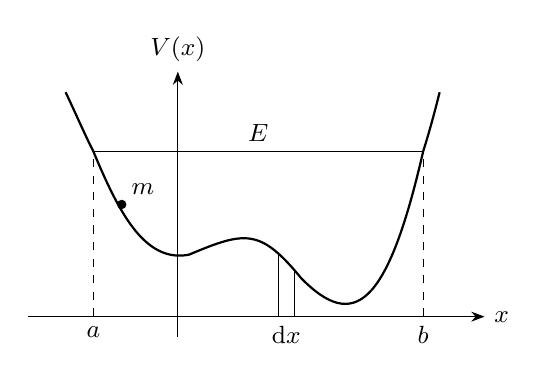
\begin{tikzpicture}[x=0.95cm,y=0.75cm,>=Stealth,font=\small]
\draw[->] (-2.7,0)--(3.4,0) node[right] {$x$};
\draw[->] (-0.7,-0.35)--(-0.7,4.15) node[above] {$V(x)$};
\draw[thick] (-2.2,3.8) .. controls (-2.05,3.4) and (-1.95,3.1) .. (-1.83,2.8)
 .. controls (-1.5,1.8) and (-1.15,0.9) .. (-0.55,1.05)
 .. controls (0.2,1.45) and (0.4,1.5) .. (0.95,0.65)
 .. controls (1.65,-0.25) and (2.1,0.15) .. (2.58,2.8)
 .. controls (2.68,3.2) and (2.75,3.55) .. (2.8,3.8);
\draw (-1.83,2.8)--(2.58,2.8) node[midway,above] {$E$};
\draw[dashed] (-1.83,0) node[below] {$a$}--(-1.83,2.8);
\draw[dashed] (2.58,0) node[below] {$b$}--(2.58,2.8);
\draw (0.65,0)--(0.65,1.05);
\draw (0.86,0)--(0.86,0.78);
\node[below] at (0.75,0) {$\dd x$};
\fill (-1.45,1.9) circle (1.7pt) node[above right] {$m$};
\end{tikzpicture}

\par\smallskip{\small 习题 1.11 图：一个势阱中的经典粒子（示意重绘）}
\end{center}
\vfill

\problem[$\ast\ast$]{1.12}
对习题 1.11（b）中的经典谐振子，若感兴趣的是动量的分布（$p=mv$），则
\begin{enumerate}
\item 求出经典几率分布 $\rho(p)$。（注意 $p$ 的取值范围是 $-\sqrt{2mE}$ 到 $+\sqrt{2mE}$。）
\item 计算 $\avg{p}$、$\avg{p^2}$ 和 $\sigma_p$。
\item 对于该系统，经典的不确定乘积 $\sigma_x\sigma_p$ 是多少？注意：一般来说，只要 $E\to0$，这个乘积值就可以足够小。但是在第 2 章将会看到，在量子力学中，简谐振子的能量不会小于 $\hbar\omega/2$，这里 $\omega=\sqrt{k/m}$ 是经典频率。在这种情况下，你对乘积 $\sigma_x\sigma_p$ 有什么看法？
\end{enumerate}
\vfill

\problem[数值实验]{1.13}
用下面的“数值实验”检验习题 1.11（b）的结果，在 $t$ 时刻谐振子的位置是
\[
x(t)=A\cos\omega t.
\]
你也可以取 $\omega=1$（设置时间标度）和 $A=1$（设置长度标度）。取 10000 个随机时间点画出 $x$ 值图，并和 $\rho(x)$ 做比较。

\textbf{提示：}使用 Mathematica，首先定义
\begin{verbatim}
x[t_] := Cos[t]
\end{verbatim}
然后构造一个位置的表格
\begin{verbatim}
snapshots = Table[x[Pi RandomReal[]], {j, 10000}]
\end{verbatim}
最后，做所获数据的柱状图：
\begin{verbatim}
Histogram[snapshots, 100, "PDF", PlotRange -> {0, 2}]
\end{verbatim}
与此同时，作密度函数 $\rho(x)$ 图，使用 \texttt{Show}，将两个叠加起来比较。
\vfill

\problem{1.14}
设 $P_{ab}(t)$ 是在 $t$ 时刻发现粒子处在区间（$a<x<b$）内的几率。
\begin{enumerate}
\item 证明：
\[
\frac{\dd P_{ab}}{\dd t}=J(a,t)-J(b,t),
\]
其中，
\[
J(x,t)=\frac{\mathrm{i}\hbar}{2m}
\left(\Psi\frac{\partial\Psi^*}{\partial x}
-\Psi^*\frac{\partial\Psi}{\partial x}\right).
\]
问 $J(x,t)$ 的单位是什么？注释：$J$ 称为几率流，因为它告诉你“流”过 $x$ 点几率的速率。若 $P_{ab}(t)$ 随时间增加，则流进该区域的一端的几率大于流出端。
\item 求出习题 1.9 中波函数的几率流。（这不是一个非常简单的例子，恐怕在以后的课程中我们会遇到更多实质性的问题。）
\end{enumerate}
\vfill

\problem{1.15}
证明：对（处在相同势场 $V(x)$ 中）任何两个同时满足薛定谔方程的（归一化）解 $\Psi_1$ 和 $\Psi_2$ 有
\[
\frac{\dd}{\dd t}\int_{-\infty}^{\infty}\Psi_1^*\Psi_2\,\dd x=0.
\]
\vfill

\problem{1.16}
（$t=0$ 时刻）粒子运动由下面波函数描述：
\[
\Psi(x,0)=\begin{cases}
A(a^2-x^2),&-a\leq x\leq a,\\
0,&\text{其他地方。}
\end{cases}
\]
\begin{enumerate}
\item 确定归一化常数 $A$。
\item $x$ 的期望值是多少？
\item $p$ 的期望值是多少？（注意：不能通过 $\avg{p}=m\,\dd\avg{x}/\dd t$ 来得到它，为什么？）
\item 求出 $x^2$ 的期望值。
\item 求出 $p^2$ 的期望值。
\item 求出 $x$ 的不确定度（即 $\sigma_x$）。
\item 求出 $p$ 的不确定度（即 $\sigma_p$）。
\item 验证所得到的结果和不确定原理一致。
\end{enumerate}
\vfill

\problem{1.17}
假设描述一个不稳定的粒子，它以“寿命”$\tau$ 自发衰变。在这种情况下，整个空间发现粒子的几率不再是常数，而是（比如说）按指数衰减：
\[
P(t)=\int_{-\infty}^{\infty}|\Psi(x,t)|^2\,\dd x=\mathrm{e}^{-t/\tau}.
\]
粗略地实现这一结果的方法如下：在式（1.24）中，我们默认假设 $V$（势能）是实数。这当然是合理的，但是它导致了式（1.27）隐含着“几率守恒”。如果在 $V$ 中添加一个虚数部分：
\[
V=V_0-\mathrm{i}\Gamma,
\]
将会怎么样？式中，$V_0$ 是真实的势能；$\Gamma$ 是一个实的常数。
\begin{enumerate}
\item 证明（取代式（1.27））存在关系
\[
\frac{\dd P}{\dd t}=-\frac{2\Gamma}{\hbar}P.
\]
\item 求出 $P(t)$，并用 $\Gamma$ 表示出粒子的寿命。
\end{enumerate}
\vfill

\problem{1.18}
粗略地讲，当粒子的德布罗意波长（$h/p$）比体系的特征长度（$d$）大时，就要涉及量子力学。在温度 $T\,\mathrm{K}$ 下粒子处于热平衡时，其平均动能是
\[
\frac{p^2}{2m}=\frac{3}{2}k_{\mathrm B}T
\]
（$k_{\mathrm B}$ 是玻尔兹曼常数，Boltzmann constant），所以对应的德布罗意波长为
\[
\lambda=\frac{h}{\sqrt{3mk_{\mathrm B}T}}.
\]
这个问题的目的是确定哪些系统必须用量子力学来处理，哪些系统可以有把握地用经典方法来描述。
\begin{enumerate}
\item \textbf{固体。}典型固体的晶格间距大约是 $d=0.3\,\mathrm{nm}$。找出固体中自由电子的量子力学温度。固体量子力学中的原子核温度低于多少（以硅为例）？原则上固体中的自由电子总是量子力学的，但原子核通常不是量子力学的。对液体也有同样的结果（原子之间的间隔和固体差不多），但是 $4\,\mathrm{K}$ 以下的氦是个例外。
\item \textbf{气体。}压强为 $p$ 的理想气体中原子的量子力学温度是多少？提示：利用理想气体定律（$pV=Nk_{\mathrm B}T$）导出原子之间的间距。
\end{enumerate}
显然（为了使气体显示量子行为）我们希望 $m$ 应当尽可能地小，而 $p$ 尽可能地大。对氦来讲，把一个大气压下的数据代入上式。问遥远宇宙中的氢（温度大约 $3\,\mathrm{K}$，原子间距大约 $1\,\mathrm{cm}$）需要用量子力学处理吗？（假设它是氢原子，不是氢分子。）
\vfill

\bookchapter{2}{定态薛定谔方程}

\problem[$\ast$]{2.1}
证明下列三个定理：
\begin{enumerate}
\item 对归一化的解，其分离变量常数 $E$ 必为实数。提示：把 $E$（式（2.7）中）写成 $E_0+\mathrm{i}\Gamma$ 的形式（$E_0$ 和 $\Gamma$ 都是实数），然后证明对任何时间 $t$，如果式（1.20）都成立，则 $\Gamma$ 必定为零。
\item 定态波函数 $\psi(x)$ 总可以取作实数（不像 $\Psi(x,t)$ 一定是复数）：这并不是说任何定态薛定谔方程的解一定是实数，而是说，如果你没有得到实数解，总可以通过这些解（具有相同能量）的线性组合得到一个实数解。所以，你总可以说薛定谔方程的解可以取作实数。提示：对于一个给定的能量 $E$，如果 $\psi(x)$ 满足式（2.5），那么 $\psi(x)$ 的共轭复数也满足；这样它们的线性组合 $\psi+\psi^*$ 和 $\mathrm{i}(\psi-\psi^*)$ 为实数解，它们同样也满足式（2.5）。
\item 如果 $V(x)$ 是偶函数（even function）（即 $V(-x)=V(x)$），那么 $\psi(x)$ 总可以取偶函数或者奇函数。提示：对于给定的能量 $E$，如果 $\psi(x)$ 满足式（2.5），那么 $\psi(-x)$ 也一定满足，所以它们的奇函数和偶函数的组合 $\psi(x)\pm\psi(-x)$ 也满足。
\end{enumerate}
\vfill

\problem[$\ast$]{2.2}
证明对于定态薛定谔方程的每一个归一化解，$E$ 必须大于 $V(x)$ 的最小值。在经典力学中，这句话对应的是什么？提示：把式（2.5）重写为
\[
\frac{\dd^2\psi}{\dd x^2}=\frac{2m}{\hbar^2}[V(x)-E]\psi;
\]
如果 $E<V_{\min}$，那么 $\psi$ 和它的二阶导数有相同的符号，论证该波函数是不可归一化的。
\vfill

\problem{2.3}
对一维无限深方势阱来说，证明在 $E=0$ 或 $E<0$ 的情况下（定态）薛定谔方程不存在可接受的（物理）解。（这是在习题 2.2 中所讨论的一般定理的一个特殊情况，但这次你要直接求解薛定谔方程，并证明其无法满足边界条件。）
\vfill

\problem[$\ast$]{2.4}
对一维无限深势阱中的第 $n$ 个定态，计算 $\avg{x}$、$\avg{x^2}$、$\avg{p}$、$\avg{p^2}$、$\sigma_x$ 和 $\sigma_p$ 的值。验证不确定原理是成立的。指出哪个状态最接近不确定原理的极限？
\vfill

\problem[$\ast$]{2.5}
一维无限深方势阱中粒子初始波函数由前两个定态波函数叠加而成：
\[
\Psi(x,0)=A[\psi_1(x)+\psi_2(x)].
\]
\begin{enumerate}
\item 归一化 $\Psi(x,0)$（即求出 $A$，如果利用 $\psi_1$ 和 $\psi_2$ 的正交归一性会使计算变得很简单。请记住，你可以认为在 $t=0$ 时波函数 $\Psi$ 是归一化的，那么在以后时间也是归一化的——如对此有疑问，在做完（b）后验证一下）。
\item 求 $\Psi(x,t)$ 和 $|\Psi(x,t)|^2$。像例题 2.1 一样，把后者用时间正弦函数表示。为简化结果起见，令 $\omega\equiv\pi^2\hbar/(2ma^2)$。
\item 计算 $\avg{x}$ 的值。注意结果是随时间振荡的。振荡的角频率是多少？振幅是多少？（如果你得到的振幅大于 $a/2$，计算一定有错。）
\item 计算 $\avg{p}$ 的值。（正如彼得·洛所讲：“当然要做，约翰尼！”）
\item 如果你对粒子的能量进行测量，可能得到的值是什么？所获得每个值的几率是多少？求出 $H$ 的期望值，并与 $E_1$ 和 $E_2$ 做比较。
\end{enumerate}
\vfill

\problem{2.6}
虽然波函数的整体相位常数都没有任何物理意义（在计算一个可观测量时可以将此抵消掉），但是在式（2.17）中系数的相对相位却起作用。例如，假定改变习题 2.5 中的 $\psi_1$ 和 $\psi_2$ 的相对相位为
\[
\Psi(x,0)=A[\psi_1(x)+\mathrm{e}^{\mathrm{i}\phi}\psi_2(x)],
\]
其中 $\phi$ 是一些常数。求解 $\Psi(x,t)$、$|\Psi(x,t)|^2$ 和 $\avg{x}$，并与前面（上题）的结果做比较。研究当 $\phi=\pi/2$ 和 $\phi=\pi$ 时的特殊情况。（对该问题的一个图示，可在脚注 9 所给出的网页中找到。）
\vfill

\problem[$\ast$]{2.7}
一维无限深势阱中的粒子初始波函数是
\[
\Psi(x,0)=\begin{cases}
Ax,&0\leq x\leq a/2,\\
A(a-x),&a/2\leq x\leq a.
\end{cases}
\]
\begin{enumerate}
\item 画出 $\Psi(x,0)$ 的草图，然后求出常数 $A$。
\item 求出 $\Psi(x,t)$。
\item 对粒子能量进行测量，得到结果为 $E_1$ 的几率是多少？
\item 利用式（2.21），求出能量的期望值。
\end{enumerate}
\vfill

\problem{2.8}
处在一维无限深（宽度为 $a$）方势阱中质量为 $m$ 的粒子，其初态为
\[
\Psi(x,0)=\begin{cases}
A,&0\leq x\leq a/2,\\
0,&a/2\leq x\leq a.
\end{cases}
\]
对于某一常数 $A$，势阱左半边的区域中（$t=0$ 时）每一处发现粒子的可能性相同。（在以后的时刻 $t$）对能量进行测量得到数值为 $\pi^2\hbar^2/(2ma^2)$ 的几率是多少？
\vfill

\problem{2.9}
对例题 2.2 中的波函数，用公式：
\[
\avg{H}=\int\Psi(x,0)^*\,\hat H\Psi(x,0)\,\dd x
\]
求在 $t=0$ 时 $H$ 的期望值。同在例题 2.3 中用式（2.21）求出的结果做比较。注意：因为 $\avg{H}$ 是不依赖时间的，所以用 $t=0$ 求解也不失其一般性。
\vfill

% 第 2 章续：由第二批习题截图录入，原书公式编号保留在文字引用中。
\problem[$\ast$]{2.10}
\begin{enumerate}
\item 构造出 $\psi_2(x)$。
\item 画出 $\psi_0$、$\psi_1$ 和 $\psi_2$ 的草图。
\item 通过直接积分，检验 $\psi_0$、$\psi_1$ 和 $\psi_2$ 的正交性。提示：如果你利用函数的奇偶性，则仅需做一个积分。
\end{enumerate}
\vfill

\problem[$\ast$]{2.11}
\begin{enumerate}
\item 通过直接积分，计算 $\psi_0$（式（2.60））和 $\psi_1$（式（2.62））态的 $\avg{x}$、$\avg{p}$、$\avg{x^2}$ 及 $\avg{p^2}$。注意：在今后涉及谐振子的问题中，如果你引入变量 $\xi=\sqrt{m\omega/\hbar}\,x$ 和常数 $\alpha=(m\omega/\pi\hbar)^{1/4}$，可以把问题简化。
\item 通过这些状态来验证不确定原理。
\item 计算这些状态的 $\avg{T}$（平均动能）和 $\avg{V}$（平均势能）。（无须再做积分。）你预期它们的和会是什么？
\end{enumerate}
\vfill

\problem[$\ast$]{2.12}
利用例题 2.5 中的方法，计算谐振子第 $n$ 个状态的 $\avg{x}$、$\avg{p}$、$\avg{x^2}$、$\avg{p^2}$ 及 $\avg{T}$。验证它们满足不确定原理。
\vfill

\problem{2.13}
处于谐振子势场中粒子的初始状态为
\[
\Psi(x,0)=A[3\psi_0(x)+4\psi_1(x)].
\]
\begin{enumerate}
\item 求出 $A$。
\item 给出 $\Psi(x,t)$ 和 $|\Psi(x,t)|^2$。如果得到的 $|\Psi(x,t)|^2$ 是经典振荡的频率，也不要太兴奋；如果我指定的是 $\psi_2(x)$ 而不是 $\psi_1(x)$，会是什么情况呢？
\item 计算 $\avg{x}$ 和 $\avg{p}$。对此波函数验证埃伦菲斯特定理（式（1.38））成立。
\item 如果你对该粒子的能量进行测量，可能有哪些值？各自出现的几率是多少？
\end{enumerate}
\vfill

\problem{2.14}
对于处在谐振子基态的粒子，在经典理论所允许范围之外发现粒子的几率是多少（精确到小数点后三位数）？

\textbf{提示：}在经典情况下，谐振子的能量为 $E=(1/2)ka^2=(1/2)m\omega^2a^2$，其中 $a$ 是振幅。所以具有能量 $E$ 的谐振子的“经典允许范围”是从 $-\sqrt{2E/(m\omega^2)}$ 到 $\sqrt{2E/(m\omega^2)}$。参考数学手册中“正态分布”或“误差函数”的数值积分，或者使用计算机进行数值计算。
\vfill

\problem{2.15}
利用递归公式（式（2.85））计算 $H_5(\xi)$ 和 $H_6(\xi)$。按照惯例选择适当常数使 $\xi$ 最高幂次的系数是 $2^n$。
\vfill

\problem[$\ast\ast$]{2.16}
在下面问题中，我们探讨关于厄米多项式的一些非常有用定理（不加证明）。
\begin{enumerate}
\item 罗德里格斯（Rodrigues formula）公式为
\[
H_n(\xi)=(-1)^n\mathrm{e}^{\xi^2}
\left(\frac{\dd}{\dd\xi}\right)^n\mathrm{e}^{-\xi^2}.
\]
利用该式推导出 $H_3$ 和 $H_4$。
\item 利用前两个厄米多项式 $H_{n-1}$ 和 $H_n$ 表示 $H_{n+1}$ 的递推关系：
\[
H_{n+1}(\xi)=2\xi H_n(\xi)-2nH_{n-1}(\xi).
\]
利用该式和（a）中的结果，求出 $H_5$ 和 $H_6$。
\item 如果你对一个 $n$ 阶多项式求导，可以得到 $n-1$ 阶的多项式。事实上，对厄米多项式有
\[
\frac{\dd H_n}{\dd\xi}=2nH_{n-1}(\xi).
\]
通过对 $H_5$ 和 $H_6$ 求导检验式（2.89）成立。
\item $H_n(\xi)$ 是母函数（generating function）$\exp(-z^2+2z\xi)$ 对 $z$ 求 $n$ 次导数后，再取 $z=0$ 时的值；换言之，它是母函数泰勒展开式中 $z^n/n!$ 项的系数：
\[
\mathrm{e}^{-z^2+2z\xi}=\sum_{n=0}^{\infty}\frac{z^n}{n!}H_n(\xi).
\]
利用这个公式求 $H_1$、$H_2$ 和 $H_3$。
\end{enumerate}
\vfill

\problem{2.17}
证明 $A\mathrm{e}^{\mathrm{i}kx}+B\mathrm{e}^{-\mathrm{i}kx}$ 和 $C\cos kx+D\sin kx$ 为 $x$ 的同一函数的等价表示形式，并用 $A$ 和 $B$ 将 $C$ 和 $D$ 表示出来，以及用 $C$ 和 $D$ 表示出 $A$ 和 $B$。注释：在量子力学中，当 $V=0$ 时，用指数形式表示一个行波来讨论自由粒子时最为方便；而正弦和余弦对应于驻波，自然它们出现在讨论无限深方势阱问题中。
\vfill

\problem{2.18}
求出自由粒子波函数式（2.95）的几率流 $J$（习题 1.14），几率流向哪个方向流动？
\vfill

\problem[$\ast\ast$]{2.19}
本题从在一个有限区间的普通傅里叶级数理论出发，引导你“证明”普朗克尔定理，并允许将有限区间扩展到无限大。
\begin{enumerate}
\item 狄利克莱定理表述为位于区间 $[-a,a]$ 的“任何”函数 $f(x)$ 都可以展开成傅里叶级数：
\[
f(x)=\sum_{n=0}^{\infty}\left[a_n\sin\left(\frac{n\pi x}{a}\right)
+b_n\cos\left(\frac{n\pi x}{a}\right)\right].
\]
证明上式可以等价写为
\[
f(x)=\sum_{n=-\infty}^{\infty}c_n\mathrm{e}^{\mathrm{i}n\pi x/a}.
\]
把 $c_n$ 用 $a_n$ 和 $b_n$ 表示出来。
\item 证明（通过适当修改傅里叶变换技巧）
\[
c_n=\frac{1}{2a}\int_{-a}^{a}f(x)\mathrm{e}^{-\mathrm{i}n\pi x/a}\,\dd x.
\]
\item 引入新变量 $k=n\pi/a$ 和 $F(k)=\sqrt{2/\pi}\,a c_n$，取代 $n$ 和 $c_n$。证明（a）和（b）变为
\begin{align*}
f(x)&=\frac{1}{\sqrt{2\pi}}\sum_{n=-\infty}^{\infty}F(k)\mathrm{e}^{\mathrm{i}kx}\Delta k,\\
F(k)&=\frac{1}{\sqrt{2\pi}}\int_{-a}^{a}f(x)\mathrm{e}^{-\mathrm{i}kx}\,\dd x,
\end{align*}
其中 $\Delta k$ 是 $n$ 变化到 $n+1$ 时 $k$ 的增量。
\item 取 $a\to\infty$ 时的极限得到普朗克尔定理。注释：鉴于它们完全不同的起源，很惊奇（也很有趣）这两个公式——一个是以 $f(x)$ 表示的 $F(k)$，另一个是以 $F(k)$ 表示的 $f(x)$——在 $a\to\infty$ 时有一个相似的结构形式。
\end{enumerate}
\vfill

\problem{2.20}
自由粒子的初始波函数为
\[
\Psi(x,0)=A\mathrm{e}^{-a|x|},
\]
其中 $A$ 和 $a$ 是正的实常数。
\begin{enumerate}
\item 归一化 $\Psi(x,0)$。
\item 求出 $\phi(k)$。
\item 以积分形式写出 $\Psi(x,t)$。
\item 讨论极限情况（$a$ 很大和 $a$ 很小）。
\end{enumerate}
\vfill

\problem[$\ast$]{2.21}
\textbf{高斯波包。}自由粒子的初始波函数为
\[
\Psi(x,0)=A\mathrm{e}^{-ax^2},
\]
其中 $A$ 和 $a$ 是常数（$a$ 是正实数）。
\begin{enumerate}
\item 归一化 $\Psi(x,0)$。
\item 求出 $\Psi(x,t)$。提示：积分式
\[
\int_{-\infty}^{\infty}\mathrm{e}^{-(ax^2+bx)}\,\dd x
\]
可以通过“配平方”的方法处理；令 $y=\sqrt{a}[x+b/(2a)]$，并注意到 $ax^2+bx=y^2-b^2/(4a)$。
\item 求出 $|\Psi(x,t)|^2$，用下面的量表示出你的结果：
\[
\omega=\sqrt{\frac{a}{1+(2\hbar at/m)^2}}.
\]
画出 $t=0$ 时和 $t$ 很大时的 $|\Psi|^2$ 草图（作为 $x$ 的函数）。定性来讲，当时间增加时，$|\Psi|^2$ 有什么变化？
\item 求出 $\avg{x}$、$\avg{p}$、$\avg{x^2}$、$\avg{p^2}$、$\sigma_x$ 和 $\sigma_p$。
\item 不确定原理成立吗？系统在什么时间 $t$ 最接近不确定原理的极限？
\end{enumerate}
\vfill

\problem[$\ast$]{2.22}
计算下列积分：
\begin{enumerate}
\item $\displaystyle\int_{-3}^{1}(x^3-3x^2+2x-1)\delta(x+2)\,\dd x$。
\item $\displaystyle\int_0^{\infty}[\cos(3x)+2]\delta(x-\pi)\,\dd x$。
\item $\displaystyle\int_{-1}^{1}\exp(|x|+3)\delta(x-2)\,\dd x$。
\end{enumerate}
\vfill

\problem{2.23}
$\delta$ 函数以积分符号表示，对任何（一般）函数 $f(x)$，如果
\[
\int_{-\infty}^{\infty}f(x)D_1(x)\,\dd x
=\int_{-\infty}^{\infty}f(x)D_2(x)\,\dd x,
\]
则涉及 $\delta$ 函数的两个表示式 $D_1(x)$ 和 $D_2(x)$ 相等。
\begin{enumerate}
\item 证明
\[
\delta(cx)=\frac{1}{|c|}\delta(x),
\]
式中，$c$ 是实常数。（一定要检验 $c$ 是负的情况。）
\item 设 $\theta(x)$ 是阶跃函数（step function）：
\[
\theta(x)=\begin{cases}1,&\text{如果 }x>0,\\0,&\text{如果 }x<0.\end{cases}
\]
（在极少数情况下，我们定义 $\theta(0)$ 为 $1/2$。）证明 $\dd\theta/\dd x=\delta(x)$。
\end{enumerate}
\vfill

\problem[$\ast\ast$]{2.24}
对式（2.132）中的波函数验证不确定原理。提示：因为 $\psi$ 的导数在 $x=0$ 处存在阶梯不连续，计算 $\avg{p^2}$ 时可能很费事。你可以利用习题 2.23（b）的结果。
\vfill

\problem{2.25}
验证 $\delta$ 函数势阱的束缚态（式（2.132））和散射态（式（2.134）和式（2.135））正交。
\vfill

\problem[$\ast$]{2.26}
$\delta(x)$ 的傅里叶变换是什么？利用普朗克尔定理，证明
\[
\delta(x)=\frac{1}{2\pi}\int_{-\infty}^{\infty}\mathrm{e}^{\mathrm{i}kx}\,\dd k.
\]
\textbf{评注：}这个公式会使任何值得尊敬的数学家都感到格外头疼。虽然这个积分明显是在 $x=0$ 处为无限大，由于被积函数一直振荡，当 $x\ne0$ 时它并不收敛（$0$ 或其他值）。有一些方法可以修补这个问题（例如，可以从 $-L$ 到 $L$ 进行积分，并把式（2.147）理解为有限积分的平均值，然后令 $L\to\infty$）。问题的根源在于 $\delta$ 函数不满足普朗克尔定理所要求的平方可积性（见脚注 44）。尽管如此，如果细心对待，式（2.147）将是极其有用的。
\vfill

\problem[$\ast\ast$]{2.27}
考虑双 $\delta$ 函数势
\[
V(x)=-\alpha[\delta(x+a)+\delta(x-a)],
\]
其中 $\alpha$ 和 $a$ 都是正常数。
\begin{enumerate}
\item 画出这个势的草图。
\item 存在有多少个束缚态？当 $\alpha=\hbar^2/(ma)$ 和 $\alpha=\hbar^2/(4ma)$ 时，求出允许的能级，并画出波函数的草图。
\item 在 $a\to0$ 和 $a\to\infty$ 的极限情况下，求束缚态能量的大小（固定 $\alpha$）？与单 $\delta$ 函数势阱的结果做比较，解释你答案合理性的原因。
\end{enumerate}
\vfill

\problem[$\ast\ast$]{2.28}
对于习题 2.27 中的势，求出其透射系数。
\vfill

\problem[$\ast$]{2.29}
分析有限深方势阱的奇束缚态的波函数。推导出允许能级所满足的超越方程，并用作图法求解。检查两种极限情况。是否总是至少存在一个奇束缚态？
\vfill

\problem{2.30}
对式（2.154）中的 $\psi(x)$ 归一化，确定常数 $D$ 和 $F$。
\vfill

\problem{2.31}
狄拉克 $\delta$ 函数可看作一个高度趋于无限、宽度趋于零、面积为 $1$ 的矩形的极限情况。证明在 $z_0\to0$ 情况下，$\delta$ 势阱（式（2.117））是个“弱”势（即便是在无限深的情况下）。把它看作有限深方势阱的一种极限情况，确定 $\delta$ 势阱的束缚态能级。验证你的结果与式（2.132）一致。同时证明在适当该极限情况下，式（2.172）将还原为式（2.144）。
\vfill

\problem{2.32}
推导出式（2.170）和式（2.171）。提示：使用式（2.168）和式（2.169），根据 $F$ 求解 $C$ 和 $D$：
\begin{align*}
C&=\left[\sin(la)+\mathrm{i}\frac{k}{l}\cos(la)\right]\mathrm{e}^{\mathrm{i}ka}F,\\
D&=\left[\cos(la)-\mathrm{i}\frac{k}{l}\sin(la)\right]\mathrm{e}^{\mathrm{i}ka}F.
\end{align*}
然后将它们代入式（2.166）和式（2.167）中。求出透射系数，并验证式（2.172）。
\vfill

\problem[$\ast\ast$]{2.33}
求出矩形势垒的透射系数（与式（2.148）相似，只不过在 $-a<x<a$ 区域内 $V(x)=+V_0>0$）。分别按照 $E<V_0$、$E=V_0$ 和 $E>V_0$ 三种情况来讨论。（注意，在这三种情况下，势垒区域内的波函数是不同的。）
\vfill

\problem{2.34}
考虑“阶梯”势：
\[
V(x)=\begin{cases}0,&x\leq0,\\V_0,&x>0.\end{cases}
\]
\begin{enumerate}
\item 对于 $E<V_0$ 的情况，计算反射系数，并讨论所得结果。
\item 计算 $E>V_0$ 时的反射系数。
\item 对于右侧势垒没有归零的势，透射系数不是简单地等于 $|F|^2/|A|^2$（$A$ 是入射波振幅，$F$ 是透射波振幅），这是由于透射波以不同的波速传播。证明对于 $E>V_0$，
\[
T=\sqrt{\frac{E-V_0}{E}}\frac{|F|^2}{|A|^2}.
\]
提示：你可以利用式（2.99）计算，或者更简洁但缺乏直观——利用几率流来算（习题 2.18）。对于 $E<V_0$，$T$ 又是多少？
\item 对 $E>V_0$ 情况，求出“阶梯”势的透射系数，并验证 $T+R=1$。
\end{enumerate}
\vfill

\problem{2.35}
质量为 $m$、动能 $E>0$ 的粒子靠近一骤降至 $V_0$ 的突变势（见下图，原书图 2.19）。
\begin{center}
% 原书图 2.19：向下阶跃势；小车仅为原题的定性类比。
\begin{tikzpicture}[x=1cm,y=0.8cm,>=Stealth,font=\small]
\draw[->] (-3.5,0)--(4,0) node[right] {$x$};
\draw[->] (0,-2.4)--(0,1.7) node[above] {$V(x)$};
\draw[very thick] (-3.3,0)--(0,0)--(0,-2)--(3.6,-2);
\node[left] at (0,-2) {$-V_0$};
\draw (-2.85,0.24) rectangle (-2.2,0.55);
\draw (-2.72,0.12) circle (0.09);
\draw (-2.33,0.12) circle (0.09);
\draw[->,thick] (-2.05,0.39)--(-1.25,0.39);
\end{tikzpicture}

\par\smallskip{\small 习题 2.35 图：从一个“悬崖”边的散射}
\end{center}
\begin{enumerate}
\item 如果 $E=V_0/3$，粒子被“反弹”回来的几率是多大？提示：与习题 2.34 相似，只不过阶梯由向上变为向下。
\item 我画这个图的目的是让你想象有一辆靠近一个悬崖的汽车，很明显汽车从悬崖边缘被弹回来的几率要比（a）中的结果小很多——除非你是兔八哥。解释为什么这个势不能正确地表示一个悬崖。提示：在图 2.19 中，当通过 $x=0$ 点时，汽车势能不连续地降到 $-V_0$；这与汽车坠落的实际情况相符吗？
\item 当一个自由的中子进入原子核时，它将遇到势能的突变，势能从外面的 $V_0=0$ 到原子核内部大约 $-12\,\mathrm{MeV}$（兆电子伏特）。假设裂变产生一个中子，其动能为 $4\,\mathrm{MeV}$，轰击上述的原子核。中子被吸收的几率是多大？由此能否触发新的裂变？提示：你可以先像（a）中计算出反射几率大小；然后用 $T=1-R$ 来求出穿透表面的几率大小。
\end{enumerate}
\vfill

\problem{2.36}
对于“中心”无限深方势阱：$V(x)=0$（$-a<x<a$），$V(x)=\infty$（其他地方），利用适当边界条件，求解定态薛定谔方程。验证你所求得的能量允许值与式（2.30）一致。证明你所得到的 $\psi$ 可以通过对式（2.28）做 $x\to(x+a)/2$ 变换而得到（并进行归一化）。画出前三个解的草图并与图 2.2 进行对比。注意势阱的宽度现在变为 $2a$。
\vfill

\problem{2.37}
处于无限深方势阱（式（2.22））中粒子初始波函数为
\[
\psi(x,0)=A\sin^3(\pi x/a)\qquad(0\leq x\leq a).
\]
求出 $A$ 和 $\psi(x,t)$，并计算作为时间的函数 $\avg{x}$。能量的期望值是多少？提示：$\sin^n\theta$ 和 $\cos^n\theta$ 可以通过重复利用三角公式化简为 $\sin(m\theta)$ 和 $\cos(m\theta)$（$m=0,1,2,\ldots,n$）的线性组合。
\vfill

\problem{2.38}
\begin{enumerate}
\item 证明：无限势阱中粒子的波函数经历一个量子恢复时间（revival time）后，恢复到初始形式。恢复时间为
\[
T=\frac{4ma^2}{\pi\hbar}.
\]
即：对于任何态（不仅仅限于定态），$\psi(x,T)=\psi(x,0)$。
\item 能量为 $E$ 的粒子在势阱壁之间往返碰撞，其经典恢复时间是多少？
\item 在什么样的能量下，两种恢复时间相等？
\end{enumerate}
\vfill

\problem{2.39}
在习题 2.7（d）中，通过对式（2.21）中各项的求和可以得到能量的期望值，但是我曾提醒你（脚注 23）不要用“老式的方法”，$\avg{H}=\int\psi(x,0)^*\hat H\psi(x,0)\,\dd x$，由于 $\psi(x,0)$ 一阶导数的不连续性，会使得二阶导数产生问题。实际上，你可以用分部积分法来做，但狄拉克 $\delta$ 函数提供了更为简洁的方法来处理这些反常问题。
\begin{enumerate}
\item 计算 $\psi(x,0)$ 一阶导数（习题 2.7），计算结果用式（2.146）中定义的阶跃函数 $\theta(x-a/2)$ 来表示。
\item 利用习题 2.23（b）得到的结果，将 $\psi(x,0)$ 的二阶导数用 $\delta$ 函数形式表示出来。
\item 求积分 $\int\psi(x,0)^*\hat H\psi(x,0)\,\dd x$，并检验其结果与前面所得结果相一致。
\end{enumerate}
\vfill

\problem{2.40}
处在谐振子势（式（2.43））中质量为 $m$ 的粒子从初态开始运动：
\[
\psi(x,0)=A\left(1-2\sqrt{\frac{m\omega}{\hbar}}\,x\right)^2
\mathrm{e}^{-m\omega x^2/(2\hbar)},
\]
其中 $A$ 为某常数。
\begin{enumerate}
\item 根据谐振子的定态，确定 $A$ 和该状态的各展开系数 $c_n$。
\item 测量粒子的能量，能得到哪些结果？对应的几率是多少？能量的期望值是多少？
\item 经过一段时间 $T$ 后的波函数是
\[
\psi(x,T)=B\left(1+2\sqrt{\frac{m\omega}{\hbar}}\,x\right)^2
\mathrm{e}^{-m\omega x^2/(2\hbar)},
\]
$B$ 为某个常数。$T$ 最小的可能值是多少？
\end{enumerate}
\vfill

\problem{2.41}
求半谐振子势所允许的能级：
\[
V(x)=\begin{cases}(1/2)m\omega^2x^2,&x>0,\\\infty,&x<0.\end{cases}
\]
（例如，这种情况表示了一个只能被拉伸而不能被压缩的弹簧。）提示：本题需要仔细思考，而具体计算很少。
\vfill

\problem{2.42}
在习题 2.21 中，已经对自由粒子静态高斯波包进行了分析。现在来对传播中的高斯波包求解同样问题，其初始波函数为
\[
\psi(x,0)=A\mathrm{e}^{-ax^2}\mathrm{e}^{\mathrm{i}lx},
\]
其中 $l$ 是一个实的常数。（建议：从 $\phi(k)$ 求 $\psi(x,t)$ 的过程中，在做积分前先做变量替换 $u=k-l$。）

波函数 $\psi(x,t)$ 具有一个高斯“波包”调制一列正弦行波结构。波包的速度是多少？行波传播的速度是多少？
\vfill

\problem[$\ast\ast$]{2.43}
在原点对称的无限深方势阱的中间存在一 $\delta$ 函数势垒，
\[
V(x)=\begin{cases}\alpha\delta(x),&-a<x<a,\\\infty,&|x|\geq a.\end{cases}
\]
求解定态薛定谔方程。分别处理波函数为偶和奇情况。没必要花时间去归一化这些波函数。求出能量的允许值（必要时可用作图法）。与没有 $\delta$ 函数存在时的情况相比，相应的能级有何不同？解释为什么奇函数解不受 $\delta$ 函数的影响。讨论 $\alpha\to0$ 和 $\alpha\to\infty$ 两种极限情况。
\vfill

\problem{2.44}
如果两个（或更多）定态薛定谔方程的不同解具有同一个能量 $E$，这些状态称为是简并的（degenerate）。例如，自由粒子态是双重简并的——一个解代表向右运动，另一个解代表向左运动。但我们从未遇到过可归一化的简并解，这并非偶然。证明如下定理：一维情况下（$-\infty<x<+\infty$），不存在简并束缚态。

\textbf{提示：}假设存在两个解 $\psi_1$ 和 $\psi_2$，具有同样的能量，$\psi_2$ 乘上 $\psi_1$ 满足的薛定谔方程，$\psi_1$ 乘上 $\psi_2$ 满足的薛定谔方程，然后两式相减，证明 $\psi_2\dd\psi_1/\dd x-\psi_1\dd\psi_2/\dd x$ 是个常数。利用归一化解在 $\pm\infty$ 应满足 $\psi\to0$ 的事实，证明这个常数事实上为零。从而得出结论 $\psi_2$ 是 $\psi_1$ 乘以一个常数因子，因此两个解是相同的。
\vfill

\problem{2.45}
证明一维势中定态的节点数目总是随能量的增加而增加。对于给定的势 $V(x)$，考虑定态薛定谔方程的两个解（实数归一化的解，$\psi_n$ 和 $\psi_m$），能量满足 $E_n>E_m$。
\begin{enumerate}
\item 证明
\[
\frac{\dd}{\dd x}\left(\frac{\dd\psi_m}{\dd x}\psi_n-\psi_m\frac{\dd\psi_n}{\dd x}\right)
=\frac{2m}{\hbar^2}(E_n-E_m)\psi_m\psi_n.
\]
\item 设 $x_1$ 和 $x_2$ 是波函数 $\psi_m(x)$ 的邻近的两个节点。证明
\[
\psi_m'(x_2)\psi_n(x_2)-\psi_m'(x_1)\psi_n(x_1)
=\frac{2m}{\hbar^2}(E_n-E_m)\int_{x_1}^{x_2}\psi_m\psi_n\,\dd x.
\]
\item 如果 $\psi_n(x)$ 在 $x_1$ 和 $x_2$ 之间不存在节点，那么在此区间内都有相同的符号。证明（b）导致矛盾。因此，在 $\psi_m(x)$ 的每对节点之间，$\psi_n(x)$ 至少有一个节点，且节点的数目随能量的增加而增加。
\end{enumerate}
\vfill

\problem{2.46}
假设质量为 $m$ 的小珠子绕周长为 $L$ 的圆环做无摩擦滑动。（这与自由粒子相似，只不过 $\psi(x+L)=\psi(x)$。）求出它的定态（并适当归一化）和相应的能量允许值。注意到对于每个能级 $E_n$（只有一个例外）都有两个相互独立的解。分别对应顺时针和逆时针运动情况，记为 $\psi_n^+(x)$ 和 $\psi_n^-(x)$。根据习题 2.44 中的定理，你如何解释此种简并性（为什么在此种情况下定理会不成立）？
\vfill

\problem[$\ast\ast$]{2.47}
注意：这是一个严格的定性问题——不允许做任何计算！考虑“双方势阱”势（见下图，原书图 2.20）。假设阱深 $V_0$ 和阱宽 $a$ 都固定，且足够大使得可以存在几个束缚态。
\begin{enumerate}
\item 对（i）$b=0$，（ii）$b\approx a$ 和（iii）$b\gg a$ 三种情况，画出基态波函数 $\psi_1$ 和第一激发态波函数 $\psi_2$ 的草图。
\item 定性描述当 $b$ 从 $0$ 变化到 $\infty$ 时，$\psi_1$ 和 $\psi_2$ 相对应的能级（$E_1$、$E_2$）的变化趋势。在同一图中画出 $E_1(b)$ 和 $E_2(b)$。
\item 双阱模型是基本的一维模型，用来描述双原子分子中电子所受到的势场作用（两个势阱代表两个原子核的吸引力）。如果两核被看作是自由移动的，它们将遵循最小能量分布。根据你在（b）中得到的结论，电子更趋向使两个核靠在一起，还是使其分离？（当然两个核之间存在排斥，不过这是另外一个问题。）
\end{enumerate}
\begin{center}
% 原书图 2.20：两个等宽等深方势阱；b 为两阱间隔。
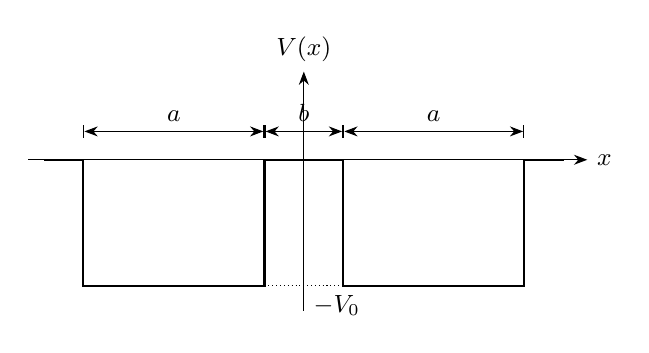
\begin{tikzpicture}[x=1cm,y=0.8cm,>=Stealth,font=\small]
\draw[->] (-3.5,0)--(3.6,0) node[right] {$x$};
\draw[->] (0,-2.4)--(0,1.4) node[above] {$V(x)$};
\draw[thick] (-3.3,0)--(-2.8,0)--(-2.8,-2)--(-0.5,-2)
 --(-0.5,0)--(0.5,0)--(0.5,-2)--(2.8,-2)--(2.8,0)--(3.3,0);
\draw[densely dotted] (-0.45,-2)--(0.45,-2);
\node[below right] at (0,-2) {$-V_0$};
\draw[|<->|] (-2.8,0.45)--(-0.5,0.45) node[midway,above] {$a$};
\draw[|<->|] (-0.5,0.45)--(0.5,0.45) node[midway,above] {$b$};
\draw[|<->|] (0.5,0.45)--(2.8,0.45) node[midway,above] {$a$};
\end{tikzpicture}

\par\smallskip{\small 习题 2.47 图：双方势阱}
\end{center}
\vfill

\problem{2.48}
处在势场中质量为 $m$ 的粒子，
\[
V(x)=\begin{cases}
\infty,&x<0,\\
-32\hbar^2/(ma^2),&0\leq x\leq a,\\
0,&x>a.
\end{cases}
\]
\begin{enumerate}
\item 存在多少个束缚态？
\item 对最高能级束缚态，粒子在阱外（$x>a$）被发现的几率是多少？
\end{enumerate}
\vfill

\problem[$\ast\ast$]{2.49}
\begin{enumerate}
\item 证明
\[
\begin{split}
\Psi(x,t)={}&\left(\frac{m\omega}{\pi\hbar}\right)^{1/4}
\exp\Biggl[-\frac{m\omega}{2\hbar}\Biggl(
x^2+\frac{x_0^2}{2}\bigl(1+\mathrm{e}^{-2\mathrm{i}\omega t}\bigr)\\
&\hspace{38mm}+\frac{\mathrm{i}\hbar t}{m}-2x_0x\mathrm{e}^{-\mathrm{i}\omega t}
\Biggr)\Biggr]
\end{split}
\]
满足谐振子的含时薛定谔方程（式（2.44））。这里 $x_0$ 是具有长度量纲的任意实数。
\item 求出 $|\Psi(x,t)|^2$，并描述波包的运动。
\item 计算 $\avg{x}$ 和 $\avg{p}$，并检验它们满足埃伦菲斯特定律（式（1.38））。
\end{enumerate}
\vfill

\problem[$\ast\ast$]{2.50}
考虑运动的 $\delta$ 函数势阱：
\[
V(x,t)=-\alpha\delta(x-vt),
\]
其中，$v$（常数）是势阱的运动速度。
\begin{enumerate}
\item 证明含时薛定谔方程有以下严格解：
\[
\Psi(x,t)=\frac{\sqrt{m\alpha}}{\hbar}
\mathrm{e}^{-m\alpha|x-vt|/\hbar^2}
\exp\left\{-\frac{\mathrm{i}}{\hbar}\left[
\left(E+\frac12mv^2\right)t-mvx\right]\right\},
\]
其中，$E=-m\alpha^2/(2\hbar^2)$ 是静止的 $\delta$ 函数的束缚态能。提示：用习题 2.23（b）所得结果，把此解代入并验证。
\item 求此状态下哈密顿量的期望值，并讨论所得结果。
\end{enumerate}
\vfill

\problem{2.51}
\textbf{自由下落。}证明
\[
\Psi(x,t)=\Psi_0\left(x+\frac12gt^2,t\right)
\exp\left[-\mathrm{i}\frac{mgt}{\hbar}\left(x+\frac16gt^2\right)\right]
\]
满足粒子在引力场
\[
V(x)=mgx
\]
中的含时薛定谔方程，这里 $\Psi_0(x,t)$ 为自由高斯波包（式（2.111））。求作为时间的函数 $\avg{x}$，并对结果进行讨论。
\vfill

\problem[$\ast\ast\ast$]{2.52}
考虑势能
\[
V(x)=-\frac{\hbar^2a^2}{m}\operatorname{sech}^2(ax),
\]
其中，$a$ 是正常数，而“$\operatorname{sech}$”代表双曲正割函数。
\begin{enumerate}
\item 画图将该势表示出来。
\item 验证该势存在基态
\[
\psi_0(x)=A\operatorname{sech}(ax),
\]
并求出基态能量。归一化 $\psi_0$，并画图表示。
\item 证明：对于任意正的能量 $E$，函数
\[
\psi_k(x)=A\left(\frac{\mathrm{i}k-a\tanh(ax)}{\mathrm{i}k+a}\right)\mathrm{e}^{\mathrm{i}kx}
\]
（一般情况下，$k=\sqrt{2mE}/\hbar$）都满足薛定谔方程。由于当 $x\to-\infty$ 时，$\tanh(ax)\to-1$，
\[
\psi_k(x)\approx A\mathrm{e}^{\mathrm{i}kx}\qquad\text{（$x$ 为大的负数），}
\]
所以，这表示从左边入射且没有伴生反射波的波（即不存在 $\exp(-\mathrm{i}kx)$ 项）。对正的较大 $x$ 值，$\psi_k(x)$ 的渐近形式是什么？对于这个势，$R$ 和 $T$ 是多少？注释：这是无反射势（reflectionless potential）的一个著名例子——每一个入射的粒子，不论其能量大小，都能够越势垒。
\end{enumerate}
\vfill

\problem{2.53}
\begingroup
\small
\setlength{\abovedisplayskip}{5pt}
\setlength{\belowdisplayskip}{5pt}
\textbf{散射矩阵。}散射理论能够以显而易见的方式推广到任意的定域势（见下图，原书图 2.21）。在左边（区域 I），$V(x)=0$，所以
\[
\psi(x)=A\mathrm{e}^{\mathrm{i}kx}+B\mathrm{e}^{-\mathrm{i}kx},
\qquad\text{其中 }k=\frac{\sqrt{2mE}}{\hbar}.
\]
\begin{center}
% 原书图 2.21 的定性重绘。区域 II 内为未指定的任意局域势。
\begin{tikzpicture}[x=0.85cm,y=0.65cm,>=Stealth,font=\scriptsize]
\draw[->] (-4.4,0)--(4.5,0) node[right] {$x$};
\draw[->] (-0.8,-0.7)--(-0.8,1.8) node[above] {$V(x)$};
\draw[thick] (-4.2,0)--(-2,0)
 .. controls (-1.7,0) and (-1.6,0.6) .. (-1.25,0.35)
 .. controls (-0.85,-0.15) and (-0.7,1.5) .. (-0.1,1.4)
 .. controls (0.5,1.5) and (0.5,-1.25) .. (1.15,-0.5)
 .. controls (1.65,0.5) and (1.65,0) .. (2.1,0)--(4.2,0);
\draw[->] (-3.9,1.1)--(-2.7,1.1) node[midway,above] {$A\mathrm{e}^{\mathrm{i}kx}$};
\draw[<-] (-3.9,0.55)--(-2.7,0.55) node[midway,below] {$B\mathrm{e}^{-\mathrm{i}kx}$};
\draw[->] (2.7,1.1)--(3.9,1.1) node[midway,above] {$F\mathrm{e}^{\mathrm{i}kx}$};
\draw[<-] (2.7,0.55)--(3.9,0.55) node[midway,below] {$G\mathrm{e}^{-\mathrm{i}kx}$};
\draw[|<->|] (-4.15,-0.95)--(-2,-0.95) node[midway,below] {区域 I};
\draw[|<->|] (-2,-0.95)--(2.1,-0.95) node[midway,below] {区域 II};
\draw[|<->|] (2.1,-0.95)--(4.15,-0.95) node[midway,below] {区域 III};
\end{tikzpicture}

\par{\footnotesize 习题 2.53 图：任意局域势的散射（除区域 II 外，$V(x)=0$）}
\end{center}
在右边（区域 III），$V(x)$ 同样为 $0$，所以
\[
\psi(x)=F\mathrm{e}^{\mathrm{i}kx}+G\mathrm{e}^{-\mathrm{i}kx}.
\]
在中间（区域 II），当然，在指定具体势之前我无法告诉你 $\psi$ 是什么，但由于薛定谔方程是一个线性二阶微分方程，通解一定具有如下形式：
\[
\psi(x)=Cf(x)+Dg(x),
\]
其中 $f(x)$ 和 $g(x)$ 是两个线性独立的特解。存在有 $4$ 个边界条件（区域 I 和区域 II 交汇处两个，区域 II 和区域 III 交汇处两个）。利用其中的两个方程可以消去 $C$ 和 $D$。其余两个用来推出用 $A$ 和 $G$ 表示的 $B$ 和 $F$：
\[
B=S_{11}A+S_{12}G,\qquad F=S_{21}A+S_{22}G.
\]
四个依赖于 $k$（从而也依赖于 $E$）的系数 $S_{ij}$ 组成一个 $2\times2$ 矩阵 $\boldsymbol S$，称为散射矩阵（scattering matrix）（简写为 $S$-矩阵）。$S$-矩阵告诉你如何以入射振幅（$A$ 和 $G$）来表示出射振幅（$B$ 和 $F$）：
\[
\begin{pmatrix}B\\F\end{pmatrix}
=\begin{pmatrix}S_{11}&S_{12}\\S_{21}&S_{22}\end{pmatrix}
\begin{pmatrix}A\\G\end{pmatrix}.
\]
从左边散射的特定情况下，$G=0$，因此，反射和透射系数为
\[
R_l=\left.\frac{|B|^2}{|A|^2}\right|_{G=0}=|S_{11}|^2,
\qquad T_l=\left.\frac{|F|^2}{|A|^2}\right|_{G=0}=|S_{21}|^2.
\]
从右边散射的情况，$A=0$，有
\[
R_r=\left.\frac{|F|^2}{|G|^2}\right|_{A=0}=|S_{22}|^2,
\qquad T_r=\left.\frac{|B|^2}{|G|^2}\right|_{A=0}=|S_{12}|^2.
\]
\begin{enumerate}
\item 构造由 $\delta$ 函数势阱（式（2.117））散射的 $S$-矩阵。
\item 构造有限深方势阱（式（2.148））的 $S$-矩阵。提示：如果你仔细分析题目的对称性，无须重新计算。
\end{enumerate}
\endgroup
\vfill

\problem[$\ast\ast\ast$]{2.54}
\textbf{传递矩阵（the transfer matrix）。}$S$-矩阵（习题 2.53）给出了出射振幅（$B$ 和 $F$）与入射振幅（$A$ 和 $G$）的关系——式（2.180）。为了某些目的利用传递矩阵 $\boldsymbol M$ 是很方便的，它可以给出势右侧波的振幅（$F$ 和 $G$）同左侧波的振幅（$A$ 和 $B$）之间的关系：
\[
\begin{pmatrix}F\\G\end{pmatrix}
=\begin{pmatrix}M_{11}&M_{12}\\M_{21}&M_{22}\end{pmatrix}
\begin{pmatrix}A\\B\end{pmatrix}.
\]
\begin{enumerate}
\item 利用 $S$-矩阵中的矩阵元求出 $M$-矩阵的四个矩阵元，反之亦然。用 $M$ 的矩阵元表示出（式（2.181）和式（2.182）中的）$R_l$、$T_l$、$R_r$ 和 $T_r$。
\item 假设有一个势是由两个孤立部分组成的（见下图，原书图 2.22），证明该势的 $M$-矩阵是由两个孤立部分势的 $M$-矩阵的乘积：
\[
\boldsymbol M=\boldsymbol M_2\boldsymbol M_1.
\]
（显然这个结论可以推广到含有任意多个部分势的情况，这说明了 $M$-矩阵的有用性。）
\item 对于在点 $a$ 处的 $\delta$ 函数散射势，构造 $M$-矩阵：
\[
V(x)=-\alpha\delta(x-a).
\]
\item 利用（b）中的方法，求双 $\delta$ 函数散射的 $M$ 矩阵：
\[
V(x)=-\alpha[\delta(x+a)+\delta(x-a)],
\]
对这个势的透射系数是什么？
\end{enumerate}
\begin{center}
% 原书图 2.22 的定性重绘：两部分势之间及外部均为 V=0。
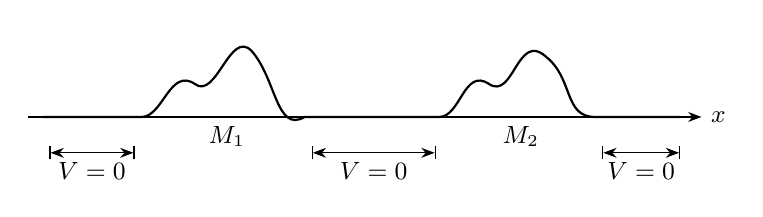
\begin{tikzpicture}[x=0.9cm,y=0.7cm,>=Stealth,font=\small]
\draw[->] (-4.5,0)--(5,0) node[right] {$x$};
\draw[thick] (-4.3,0)--(-2.9,0)
 .. controls (-2.6,0) and (-2.5,0.9) .. (-2.15,0.6)
 .. controls (-1.85,0.3) and (-1.65,1.6) .. (-1.35,1.2)
 .. controls (-1,0.7) and (-1,-0.3) .. (-0.6,0)--(1.3,0)
 .. controls (1.6,0) and (1.65,0.9) .. (2,0.6)
 .. controls (2.35,0.3) and (2.4,1.55) .. (2.8,1.1)
 .. controls (3.2,0.7) and (3.05,0) .. (3.5,0)--(4.7,0);
\node[below] at (-1.7,0) {$M_1$};
\node[below] at (2.45,0) {$M_2$};
\draw[|<->|] (-4.2,-0.65)--(-3,-0.65) node[midway,below] {$V=0$};
\draw[|<->|] (-0.5,-0.65)--(1.25,-0.65) node[midway,below] {$V=0$};
\draw[|<->|] (3.6,-0.65)--(4.7,-0.65) node[midway,below] {$V=0$};
\end{tikzpicture}

\par\smallskip{\small 习题 2.54 图：含有两个孤立部分的势}
\end{center}
\vfill

% 第 2 章续：第三批图片，2.55--2.64。
\problem[$\ast\ast$；数值实验]{2.55}
利用“摇摆狗尾”方法，求出谐振子的基态能级，并保留 5 位有效数字。也就是说，用数值法求解方程（2.73），通过不断改变 $K$ 值，直到 $\xi$ 很大时，能得到一个趋于零的波函数。在 Mathematica 中，适当的输入程序语句为：
\begingroup\small
\begin{verbatim}
Plot[
  Evaluate[
    u[x] /.
      NDSolve[
        {u''[x] - (x^2 - K)*u[x] == 0,
         u[0] == 1, u'[0] == 0},
        u[x], {x, 0, b}
      ]
  ],
  {x, a, b}, PlotRange -> {c, d}
]
\end{verbatim}
\endgroup
（这里 $(a,b)$ 是图中水平方向取值范围，$(c,d)$ 是竖直方向的取值范围——起始值分别是：$a=0$，$b=10$，$c=-10$，$d=10$。）我们知道正确解满足 $K=2n+1$，所以可以从“猜测的值”$K=0.9$ 开始。注意观察波函数“尾部”的变化行为。再尝试 $K=1.1$，注意“尾部”的快速翻转。正确解就位于这两个值之间的某处。通过调整使两端的 $K$ 值差越来越小，使波函数尾部归零。这样做的时候，你也可以调整 $a$、$b$、$c$ 和 $d$ 的值，使零点出现在交叉点。
\vfill

\problem[数值实验]{2.56}
利用习题 2.55 中的“摇摆狗”方法求出谐振子的前 3 个激发态的能级（保留五位有效数字）。对第一（和第三）激发态需要设定 $u(0)=0$，$u'(0)=1$。
\vfill

\problem[数值实验]{2.57}
利用“摇摆狗”方法求出无限深方势阱中的前 4 个能级（保留五位有效数字）。提示：参看习题 2.55，对微分方程做适当改变。本题需要寻找的条件是 $u(1)=0$。
\vfill

\problem{2.58}
在单价金属固体中，每个原子的一个电子在固体中自由运动。是什么把固体结合在一起的？为何他们不散落成一堆单独的原子？显然是聚集结构的能量一定比每个孤立原子的总能量小。本题目给出关于金属结合的一个粗略但具有启发性的解释。
\begin{enumerate}
\item 把孤立金属原子看成是其一个电子处在宽度为 $a$ 的无限深方势阱中的基态（见下图（a），原书图 2.23a），估计 $N$ 个孤立原子的能量。
\item 当这些原子聚集一起形成金属，可以看作是 $N$ 个电子位于宽度为 $Na$ 的无限深势阱中运动（见下图（b），原书图 2.23b）。由于泡利不相容原理（将在第 5 章讨论），每个允许的能级只能有一个电子（如果考虑自旋，为两个电子；先忽略自旋）。这样一个系统的最低能量是多少？
\item 上述两种情况下的能量差就是金属的内聚能（cohesive energy）——也就是把金属撕裂成孤立原子所需要的能量。在 $N$ 很大的极限情况下，求出每个原子的内聚能。
\item 金属中典型原子间的距离是几个埃（比如，$a\approx4\,\text{\AA}$），在此模型中每个原子的内聚能的数值是多少（测量值在 $2\sim4\,\mathrm{eV}$ 的范围内）？
\end{enumerate}
\begin{center}
% 原书图 2.23 的定性重绘：孤立的 N 个阱与一个共同势阱。
\begin{tikzpicture}[x=0.85cm,y=0.6cm,>=Stealth,font=\small]
\foreach \x in {0,1.5,3,6.5}{
  \draw[thick] (\x,2.1)--(\x,0)--(\x+0.95,0)--(\x+0.95,2.1);
  \draw (\x+0.48,0.08) circle (0.065);
}
\node at (5.15,0.8) {$\cdots$};
\draw[|<->|] (0,-0.4)--(0.95,-0.4) node[midway,below] {$a$};
\node at (3.75,-0.65) {（a）};
\begin{scope}[yshift=-3.2cm]
\draw[thick] (0,2.1)--(0,0)--(7.45,0)--(7.45,2.1);
\foreach \x in {0.3,1.05,1.8,2.55,3.3,5.2,5.95,6.7}{
  \draw (\x,0.08) circle (0.065);
}
\node at (4.2,0.12) {$\cdots$};
\draw[|<->|] (0,-0.4)--(7.45,-0.4) node[midway,below] {$Na$};
\node at (3.75,-1.2) {（b）};
\end{scope}
\end{tikzpicture}

\par\smallskip{\small 习题 2.58 图：（a）独立势阱；（b）宽度为 $Na$ 的共同势阱}
\end{center}
\vfill

\problem[$\ast$；数值实验]{2.59}
\textbf{“弹跳球”。}假设
\[
V(x)=\begin{cases}mgx,&x>0,\\\infty,&x\leq0.\end{cases}
\]
\begin{enumerate}
\item 求解该势的定态薛定谔方程。提示：首先把方程转换成无量纲形式：
\[
-y''(z)+zy(z)=\varepsilon y(z),
\]
通过令 $z=\alpha x$ 和 $y(z)=(1/\sqrt{\alpha})\psi(x)$（$\sqrt{\alpha}$ 使得若 $\psi(x)$ 对于 $x$ 是归一化的，则 $y(z)$ 对于 $z$ 也是归一化的）。常数 $\alpha$ 和 $\varepsilon$ 的值是多少？事实上，也可以令 $\alpha\to1$——这等同于方便选择一个长度单位。求出方程的一般解（Mathematica 中的 \texttt{DSolve} 指令可以实现）。当然，结果是两个（可能是不熟悉的）波函数的线性组合。在 $-15<z<5$ 区间内，画出两个波函数。其中的一个波函数在 $z$ 较大时明显地不趋于零（更确切地说，它不可以归一化），因此，舍弃它。$\varepsilon$ 的允许值（也是 $E$ 的允许值）由条件 $\psi(0)=0$ 确定。数值计算基态能量 $\varepsilon_1$ 和第 10 个能级 $\varepsilon_{10}$（Mathematica 中的 \texttt{FindRoot} 指令可以实现）。给出其相应的归一化因子。在 $0\leq x\leq16$ 区间内，画出 $\psi_1(x)$ 和 $\psi_{10}(x)$。仅仅作为检验，确定 $\psi_1(x)$ 和 $\psi_{10}(x)$ 是正交的。
\item 对于这两个状态，求出其不确定度 $\sigma_x$ 和 $\sigma_p$，并验证符合不确定原理。
\item 求位于高度 $x$ 位置的 $\dd x$ 区间内，发现该球的几率是 $\rho_Q(x)\,\dd x=|\psi(x)|^2\,\dd x$。最接近的经典类比是弹性球在高度 $x$ 位置处 $\dd x$ 区间所经历时间的分数（见习题 1.11）。证明其为
\[
\rho_C(x)\,\dd x=\frac{mg}{2\sqrt{E(E-mgx)}}\,\dd x,
\]
或者，以我们的单位（$\alpha=1$），
\[
\rho_C(x)=\frac{1}{2\sqrt{\varepsilon(\varepsilon-x)}}.
\]
在 $0\leq x\leq12.5$ 区间内，画出态 $\psi_{10}(x)$ 的 $\rho_Q(x)$ 和 $\rho_C(x)$ 的叠加图形（Mathematica 中的 \texttt{Show} 命令），并讨论你的结果。
\end{enumerate}
\vfill

\problem[$\ast\ast\ast$；数值实验]{2.60}
\begingroup\small
\setlength{\abovedisplayskip}{5pt}
\setlength{\belowdisplayskip}{5pt}
\textbf{$1/x^2$ 势。}假设
\[
V(x)=\begin{cases}-\alpha/x^2,&x>0,\\\infty,&x\leq0,\end{cases}
\]
这里 $\alpha$ 是具有适当量纲的正常数。我们希望找到其束缚态——求解能量为负值的（$E<0$）定态薛定谔方程：
\[
-\frac{\hbar^2}{2m}\frac{\dd^2\psi}{\dd x^2}-\frac{\alpha}{x^2}\psi=E\psi.
\]
\begin{enumerate}
\item 讨论基态能量 $E_0$：从量纲的角度证明，不可能存在 $E_0$ 的公式——无法（从可以利用的常数 $m$、$\hbar$ 和 $\alpha$）来构造一个具有能量单位的物理量。
\item 简便起见，式（2.190）重写为
\[
\frac{\dd^2\psi}{\dd x^2}+\frac{\beta}{x^2}\psi=\kappa^2\psi,
\qquad\text{这里 }\beta=\frac{2m\alpha}{\hbar^2},\quad
\kappa=\frac{\sqrt{-2mE}}{\hbar}.
\]
证明：如果 $\psi(x)$ 满足上述方程，能量为 $E$，那么，对任意的正数 $\lambda$，$\psi(\lambda x)$ 也一样满足，且能量为 $E'=\lambda^2E$。（这是个灾难。如果真的存在解，那么也就存在对任何负能量都成立的一个解。与我们遇到过的方势阱、谐振子和所有的其他势阱不一样，不存在离散的许可状态——且没有基态。一个没有最低的能量允许值的基态的系统——将是极其不稳定，级联式的能级下降，在下落时释放无限的能量。它也许可以解决我们的能源问题，但在这个过程中我们都将被灼伤。）好的，也许根本就没有解……
\item 证明（利用计算机来解决其余部分）
\[
\psi_\kappa(x)=A\sqrt{x}\,K_{\mathrm{i}g}(\kappa x)
\]
满足式（2.191）（这里 $K_{\mathrm{i}g}$ 是 $\mathrm{i}g$ 阶修正的贝塞耳函数，且 $g=\sqrt{\beta-1/4}$）。对 $g=4$，画出该波函数（图中你不妨令 $\kappa=1$，这只是设置长度的标度）。注意当 $x\to0$ 和 $x\to\infty$ 时，$\psi_\kappa$ 趋近零，所以它是可归一化的：确定 $A$ 的值。\footnote{只要 $g$ 是实数——也就是说，在 $\beta>1/4$ 的条件下，$\psi_\kappa(x)$ 就是可归一化的。}前述的节点数等于能量较低的状态数这一旧规则会变得如何？无论能量大小（即 $\kappa$ 的大小），这个函数有无限个节点，我想这是一致的，因为对任意的 $E$，都存在无限多的比其能量更低的态。
\item 这个势函数几乎混淆了我们所期望的一切。问题是这个势在 $x\to0$ 时，变化得太剧烈。如果你把这个“砖墙”移动一点，
\[
V(x)=\begin{cases}-\alpha/x^2,&x>\epsilon>0,\\\infty,&x\leq\epsilon,\end{cases}
\]
突然它们就变得正常了。对于 $g=4$ 和 $\epsilon=1$，在 $x=0$ 至 $x=6$ 范围内画出基态波函数（你首先需要确定合适的 $\kappa$ 值），注意我们引入了具有长度的量纲的新参数（$\epsilon$），因此，在（a）中的争论不在讨论范围之内。证明：对无量纲变量 $\beta$ 的一些函数 $f$，基态能具有形式
\[
E_0=-\frac{\alpha}{\epsilon^2}f(\beta).
\]
\end{enumerate}
\endgroup
\vfill

\problem[$\ast\ast\ast$；数值实验]{2.61}
\begingroup\small
\setlength{\abovedisplayskip}{4pt}
\setlength{\belowdisplayskip}{4pt}
获得势阱能级允许值的一种数值方法是，通过变量 $x$ 的离散化把薛定谔方程变成矩阵方程。在等间距的点 $\{x_j\}$ 中划分出相关间隔，$x_{j+1}-x_j=\Delta x$，令 $\psi_j=\psi(x_j)$（同样，$V_j=V(x_j)$），那么
\[
\frac{\dd\psi}{\dd x}\approx\frac{\psi_{j+1}-\psi_j}{\Delta x},\qquad
\frac{\dd^2\psi}{\dd x^2}\approx
\frac{(\psi_{j+1}-\psi_j)-(\psi_j-\psi_{j-1})}{(\Delta x)^2}
=\frac{\psi_{j+1}-2\psi_j+\psi_{j-1}}{(\Delta x)^2}.
\]
（随着 $\Delta x$ 的减少，这种近似将逐步改善。）离散的薛定谔方程是
\[
-\frac{\hbar^2}{2m}\left(\frac{\psi_{j+1}-2\psi_j+\psi_{j-1}}{(\Delta x)^2}\right)
+V_j\psi_j=E\psi_j,
\]
或者
\[
-\lambda\psi_{j+1}+(2\lambda+V_j)\psi_j-\lambda\psi_{j-1}=E\psi_j,
\qquad\text{这里 }\lambda=\frac{\hbar^2}{2m(\Delta x)^2}.
\]
矩阵形式
\[
\boldsymbol H\boldsymbol\Psi=E\boldsymbol\Psi.
\]
这里（令 $v_j=V_j/\lambda$）
\[
\boldsymbol H=\lambda
\begin{pmatrix}
\ddots&&&&&\\
&-1&2+v_{j-1}&-1&0&0\\
&0&-1&2+v_j&-1&0\\
&0&0&-1&2+v_{j+1}&-1\\
&&&&&\ddots
\end{pmatrix},
\qquad
\boldsymbol\Psi=\begin{pmatrix}\vdots\\\psi_{j-1}\\\psi_j\\\psi_{j+1}\\\vdots\end{pmatrix}.
\]
\textbf{整理注：}原图式（2.199）的矩阵前未写整体因子 $\lambda$；此处按式（2.197）补入，使矩阵方程与差分方程、能量量纲一致。

（下面将会看到，$H$ 的左上角和右下角是什么依赖于边界条件。）很明显，能量允许值是矩阵 $H$ 的本征值（或者说，$\Delta x\to0$ 的极限）。

将这种方法应用于无限深方势阱。把 $0\leq x\leq a$ 区间分成 $N+1$ 个相等的部分（所以 $\Delta x=a/(N+1)$），令 $x_0=0$ 和 $x_{N+1}=a$。边界条件 $\psi_0=\psi_{N+1}=0$，有
\[
\boldsymbol\Psi=\begin{pmatrix}\psi_1\\\vdots\\\psi_N\end{pmatrix}.
\]
\begin{enumerate}
\item 对 $N=1$、$N=2$ 和 $N=3$，构造 $H$ 的 $N\times N$ 矩阵。（对于特殊情况 $j=1$ 和 $j=N$，确保能够正确地表示出式（2.197）。）
\item 对这 3 种情况，“手动”求出 $H$ 的本征值，并与精确的能级允许值（式（2.30））作比较。
\item 对 $N=10$ 和 $N=100$，利用计算机数值求解出最低的 5 个能级本征值（Mathematica 中 \texttt{Eigenvalues} 软件包可以处理这个问题），并与精确解比较。
\item 画出（“手动”）$N=1$、$N=2$ 和 $N=3$ 时的本征矢，用计算机（\texttt{Eigenvectors} 软件包）画出 $N=10$ 和 $N=100$ 时的前 3 个本征矢。
\end{enumerate}
\endgroup
\vfill

\problem[$\ast\ast$；数值实验]{2.62}
假设无限深方势阱的底部不是平坦的（$V(x)=0$），而是
\[
V(x)=500V_0\sin\left(\frac{\pi x}{a}\right),
\qquad\text{这里 }V_0=\frac{\hbar^2}{2ma^2}.
\]
使用习题 2.61 中的数值方法求出其前 3 个能量允许值，并画出其相应的波函数（取 $N=100$）。
\vfill

\problem{2.63}
\begingroup\small
\setlength{\abovedisplayskip}{4pt}
\setlength{\belowdisplayskip}{4pt}
玻尔兹曼方程
\[
P(n)=\frac{1}{Z}\mathrm{e}^{-\beta E_n},\qquad
Z=\sum_n\mathrm{e}^{-\beta E_n},\qquad\beta\equiv\frac{1}{k_{\mathrm B}T},
\]
给出系统在温度为 $T$ 时，处在状态 $n$（能量为 $E_n$）的几率（$k_{\mathrm B}$ 是玻尔兹曼常量）。注释：这里的几率指的是随机热分布，与量子的不确定没有任何关系。只有在能量 $E_n$ 量子化情况下，该问题才涉及量子力学。
\begin{enumerate}
\item 说明系统能量的热平均可以表示为
\[
\overline E=\sum_n E_nP(n)=-\frac{\partial}{\partial\beta}\ln Z.
\]
\item 对于简单的量子谐振子，指标 $n$ 就是量子数，且 $E_n=(n+1/2)\hbar\omega$。证明在这种情况下，配分函数（partition function）$Z$ 为
\[
Z=\frac{\mathrm{e}^{-\beta\hbar\omega/2}}{1-\mathrm{e}^{-\beta\hbar\omega}}.
\]
你需要对一个几何级数序列求和。顺便提及，对于经典谐振子，可以证明 $Z_{\text{经典}}=2\pi/(\omega\beta)$。
\item 利用（a）和（b）的结果，证明：对于量子谐振子
\[
\overline E=\left(\frac{\hbar\omega}{2}\right)
\frac{1+\mathrm{e}^{-\beta\hbar\omega}}{1-\mathrm{e}^{-\beta\hbar\omega}}.
\]
对经典谐振子，同样的推理可以得到 $\overline E_{\text{经典}}=1/\beta=k_{\mathrm B}T$。
\item 由 $N$ 个原子组成的晶体可以看成 $3N$ 个振子的集合（每个原子和其周围沿 $x$、$y$ 和 $z$ 方向的 6 个最近邻原子由弹簧连接，两端的原子共用这些弹簧），因而晶体的（每个原子）热容（heat capacity）是
\[
C=3\frac{\partial\overline E}{\partial T}.
\]
证明（在此模型下）
\[
C=3k_{\mathrm B}\left(\frac{\theta_E}{T}\right)^2
\frac{\mathrm{e}^{\theta_E/T}}{(\mathrm{e}^{\theta_E/T}-1)^2},
\]
这里 $\theta_E=\hbar\omega/k_{\mathrm B}$ 是所谓的爱因斯坦温度（Einstein temperature）。利用 $\overline E$ 的经典表示式，同样的推理可以得到 $C_{\text{经典}}=3k_{\mathrm B}$，它和温度无关。
\item 画出 $C/k_{\mathrm B}$--$T/\theta_E$ 草图，你的结果看起来和图 2.24 中的金刚石的数据相似，和经典预言的结果完全不同。
\end{enumerate}
\begin{center}
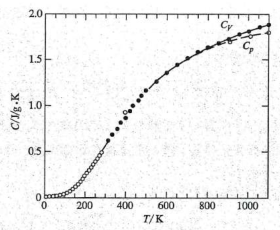
\includegraphics[height=43mm,keepaspectratio]{figures/fig_2_63_scan.png}
\par{\footnotesize 习题 2.63 图：金刚石的比热（原书图 2.24，原图摘录）}
\par{\footnotesize 原图注明来源：\textit{Semiconductor on NSM}。}
\end{center}
\endgroup
\vfill

\problem{2.64}
勒让德微分方程（Legendre's differential equation）为
\[
(1-x^2)\frac{\dd^2f}{\dd x^2}-2x\frac{\dd f}{\dd x}+l(l+1)f=0,
\]
这里 $l$ 是一些（非负）实数。
\begin{enumerate}
\item 假定存在一个幂级数解
\[
f(x)=\sum_{n=0}^{\infty}a_nx^n,
\]
给出常数 $a_n$ 的递推关系。
\item 论证除非这个级数被截断（只有当 $l$ 是整数时才会发生），方程的解在 $x=1$ 时将会发散。
\item 当 $l$ 是一个整数时，两个线性独立解中的一个级数序列会被截断（根据 $l$ 的奇偶不同，要么 $f_{\text{偶}}$，要么 $f_{\text{奇}}$），这些解称为勒让德多项式（Legendre polynomials）$P_l(x)$。利用递推关系求出 $P_0(x)$、$P_1(x)$、$P_2(x)$ 和 $P_3(x)$。答案用 $a_0$ 或者 $a_1$ 表示。
\end{enumerate}
\vfill

\bookchapter{3}{形式理论}

\problem{3.1}
\begin{enumerate}
\item 证明全体平方可积函数集构成一个矢量空间（参考 A.1 节中的定义）。提示：要点是证明两个平方可积函数之和也是平方可积的。利用式（3.7）。全体可归一化的函数集构成矢量空间吗？
\item 证明式（3.6）中的积分满足内积条件（A.2 节）。
\end{enumerate}
\vfill

\problem[$\ast$]{3.2}
\begin{enumerate}
\item 对 $\nu$ 范围取什么时，在 $(0,1)$ 区间内的函数 $f(x)=x^\nu$ 在希尔伯特空间中？假设 $\nu$ 是实数，但不必是正数。
\item 对于 $\nu=1/2$ 的特定情况，$f(x)$ 还在希尔伯特空间吗？$xf(x)$ 呢？$(\dd/\dd x)f(x)$ 呢？
\end{enumerate}
\vfill

\problem[$\ast$]{3.3}
证明如果对于所有的 $h$（希尔伯特空间中）都有
\[
\langle h\mid\hat Qh\rangle=\langle\hat Qh\mid h\rangle,
\]
则对于所有的 $f$ 和 $g$ 也有
\[
\langle f\mid\hat Qg\rangle=\langle\hat Qf\mid g\rangle
\]
（也就是，两种“厄米算符”的定义是等价的——式（3.16）和式（3.17））。提示：先令 $h=f+g$，然后再令 $h=f+\mathrm{i}g$。
\vfill

\problem{3.4}
\begin{enumerate}
\item 证明两个厄米算符之和仍是厄米算符。\footnote{在一个有限维的空间，厄米算符用厄米矩阵表示。厄米矩阵等于其厄米共轭：$\boldsymbol T=\boldsymbol T^\dagger\equiv\widetilde{\boldsymbol T}^{\,*}$。假如你对此不熟悉，请参阅附录。}
\item 假设 $\hat Q$ 是厄米的，且 $\alpha$ 为复数，$\alpha$ 在什么条件下 $\alpha\hat Q$ 也是厄米的？
\item 在什么条件下两个厄米算符的积也是厄米算符？
\item 证明位置算符（$\hat x=x$）和哈密顿算符
\[
\hat H=-\frac{\hbar^2}{2m}\frac{\dd^2}{\dd x^2}+V(x)
\]
是厄米算符。\footnote{正如我第 1 章中提到的，存在平方可积的极端函数，但在无限远处并不为 $0$。然而，在物理学中并不存在这些函数。如果你担心这一点，我们可以简单限制算符的域，把它们排除在外。在有限区间中，你要特别小心边界项，一个算符在 $(-\infty,+\infty)$ 区间是厄米算符，在 $(0,\infty)$ 或 $(-\pi,+\pi)$ 区间上并非一定是厄米算符。对无限深方势阱，最安全的是认为这些波函数位于无限长直线上——它们只不过是恰巧在 $(0,a)$ 之外等于零。参看习题 3.48。}
\end{enumerate}
\vfill

\problem{3.5}
\begin{enumerate}
\item 求出 $x$、$\mathrm{i}$ 和 $\dd/\dd x$ 的厄米共轭算符。
\item 证明：
\[
(\hat Q\hat R)^\dagger=\hat R^\dagger\hat Q^\dagger
\quad\text{（注意颠倒顺序），}\qquad
(\hat Q+\hat R)^\dagger=\hat R^\dagger+\hat Q^\dagger,
\]
以及对复数 $c$ 有 $(c\hat Q)^\dagger=c^*\hat Q^\dagger$。
\item 构建 $a_\pm$ 的厄米共轭算符（式（2.48））。
\end{enumerate}
\vfill

\problem{3.6}
考虑算符 $\hat Q=\dd^2/\dd\phi^2$，其中 $\phi$ 是极坐标中的方位角（同例题 3.1），且函数同样遵从式（3.26）。$\hat Q$ 是厄米算符吗？求出它的本征函数和本征值。$\hat Q$ 的谱是什么？这个谱是简并的吗？
\vfill

\problem{3.7}
\begin{enumerate}
\item 假设 $f(x)$ 和 $g(x)$ 是算符 $\hat Q$ 的两个具有相同本征值 $q$ 的本征函数。证明任何 $f$ 和 $g$ 的线性组合也是 $\hat Q$ 的本征函数，且本征值为 $q$。
\item 验证 $f(x)=\exp(x)$ 与 $g(x)=\exp(-x)$ 是算符 $\dd^2/\dd x^2$ 具有相同本征值的两个本征函数。
\end{enumerate}
由 $f$ 和 $g$ 的线性组合构造两个波函数，使在 $(-1,1)$ 范围内它们是正交的。
\vfill

\problem{3.8}
\begin{enumerate}
\item 验证例题 3.1 中厄米算符的本征值是实数。证明具有不同本征值的本征函数正交。
\item 对习题 3.6 中的算符做同样的验证。
\end{enumerate}
\vfill

% 第四批图片：仅录入已提供的题目；缺 3.17、3.23--3.30。
\problem{3.9}
\begin{enumerate}
\item 列举一个第 2 章中哈密顿量（谐振子除外），它仅有离散谱。
\item 列举一个第 2 章中的哈密顿量（自由粒子除外），它仅有连续谱。
\item 列举一个第 2 章中的哈密顿量（有限深方势阱除外），它既有离散谱又有连续谱。
\end{enumerate}
\vfill

\problem{3.10}
无限深方势阱的基态是动量的本征函数吗？如果是的话，它的动量是多少？如果不是，给出理由？（进一步的讨论参见习题 3.34。）
\vfill

\problem{3.11}
对处于谐振子基态的粒子，求出其动量空间波函数 $\Phi(p,t)$。对该粒子的动量进行测量，得到其结果处在经典范围（具有相同能量）以外的几率是多大（精确到两位数）？提示：数值计算部分可查阅数学手册中“正态分布”或“误差函数”，或使用 Mathematica 软件。
\vfill

\problem{3.12}
由式（2.101）引入的函数 $\phi(k)$ 求出自由粒子的 $\Phi(p,t)$。证明：对于自由粒子，$|\Phi(p,t)|^2$ 和时间无关。评注：对于自由粒子而言，$|\Phi(p,t)|^2$ 和时间无关是该系统动量守恒的一个表现。
\vfill

\problem[$\ast$]{3.13}
证明
\[
\avg{x}=\int\Phi^*\left(\mathrm{i}\hbar\frac{\partial}{\partial p}\right)\Phi\,\dd p.
\]
\textbf{提示：}注意到 $x\exp(\mathrm{i}px/\hbar)=-\mathrm{i}\hbar(\partial/\partial p)\exp(\mathrm{i}px/\hbar)$，并利用式（2.147）。则在动量空间中，位置算符是 $\mathrm{i}\hbar\partial/\partial p$。更为普遍地有
\[
\avg{Q(x,p,t)}=
\begin{cases}
\displaystyle\int\Psi^*\hat Q\left(x,-\mathrm{i}\hbar\frac{\partial}{\partial x},t\right)\Psi\,\dd x,
&\text{在位置空间；}\\[10pt]
\displaystyle\int\Phi^*\hat Q\left(\mathrm{i}\hbar\frac{\partial}{\partial p},p,t\right)\Phi\,\dd p,
&\text{在动量空间。}
\end{cases}
\]
原则上，你们可以像在位置空间一样在动量空间做所有的计算（虽然不总是那么容易）。

\textbf{整理注：}原图提示的文字将动量空间位置算符写成负号，与同图式（3.57）、（3.58）不符；此处统一为正号 $\mathrm{i}\hbar\partial/\partial p$。
\vfill

\problem[$\ast$]{3.14}
\begin{enumerate}
\item 证明下列对易关系等式：
\begin{align*}
[\hat A+\hat B,\hat C]&=[\hat A,\hat C]+[\hat B,\hat C],\\
[\hat A\hat B,\hat C]&=\hat A[\hat B,\hat C]+[\hat A,\hat C]\hat B.
\end{align*}
\item 证明
\[
[x^n,\hat p]=\mathrm{i}\hbar n x^{n-1}.
\]
\item 对可以进行泰勒级数展开的任意函数 $f(x)$，更普遍地证明
\[
[f(x),\hat p]=\mathrm{i}\hbar\frac{\dd f}{\dd x}.
\]
\item 对简谐振子，证明
\[
[\hat H,\hat a_\pm]=\pm\hbar\omega\hat a_\pm.
\]
提示：利用式（2.54）。
\end{enumerate}
\vfill

\problem[$\ast$]{3.15}
对于位置（$A=x$）的不确定性和能量（$B=p^2/(2m)+V$）的不确定性，证明著名的“（你的雅号）不确定原理”：
\[
\sigma_x\sigma_H\geq\frac{\hbar}{2m}|\avg{p}|.
\]
对于定态，它告诉不了你多少——为什么不能？
\vfill

\problem{3.16}
证明两个非对易算符不能拥有完备的共同本征函数集。提示：证明如果 $\hat P$ 和 $\hat Q$ 拥有完备的共同本征函数集，则对于希尔伯特空间的任意函数有 $[\hat P,\hat Q]f=0$。
\vfill

% 习题 3.17 未在本批图片中出现。
\problem{3.18}
在下列特殊情况中应用式（3.73）：（a）$Q=1$；（b）$Q=H$；（c）$Q=x$；（d）$Q=p$。对每种情况，特别是参考式（1.27）、式（1.33）、式（1.38）和能量守恒（式（2.21）后的注释），对你的结果进行讨论。
\vfill

\problem{3.19}
用式（3.73）（或者习题 3.18（c）和（d））证明：
\begin{enumerate}
\item 对于描述自由粒子（$V(x)=0$）的任意归一化波包，$\avg{x}$ 以恒定速度运动（这是牛顿第一定律的量子类似物）。注释：虽然采用习题 2.42 中的高斯波包来证明，但结论是普适的。
\item 对于处于谐振子（$V(x)=\frac12m\omega^2x^2$）势场中的任意波包，$\avg{x}$ 以经典频率振动。注释：虽然采用习题 2.49 中的高斯波包来证明，但结论是普适的。
\end{enumerate}
\vfill

\problem{3.20}
对习题 2.5 中的波函数和可观测量 $x$，通过精确计算 $\sigma_H$、$\sigma_x$ 和 $\dd\avg{x}/\dd t$ 来验证能量--时间不确定原理。
\vfill

\problem{3.21}
对习题 2.42 中的自由粒子波包和可观测量 $x$，通过精确计算 $\sigma_H$、$\sigma_x$ 和 $\dd\avg{x}/\dd t$ 来验证能量--时间不确定原理。
\vfill

\problem{3.22}
证明当所涉及的可观测量为 $x$ 时，能量--时间不确定原理还原为在习题 3.15 证明的不确定原理。
\vfill

% 第五批图片补齐 3.23--3.30，按教材题号插入。
% 补录第五批图片；由 chapter3_09_49.tex 在 3.22 后按题号插入。
\problem{3.23}
证明投影算符等幂（idempotent）：$\hat P^2=\hat P$。求 $\hat P$ 的本征值，并描述其本征矢量。
\vfill

\problem{3.24}
证明：若 $\hat Q$ 是厄米算符，则在任意正交基内所表示的矩阵元满足 $Q_{mn}=Q_{nm}^*$。也就是说，相应的矩阵等于其厄米共轭。\footnote{根据式（3.20），注意到 $\langle\hat Qf|=\langle f|\hat Q^\dagger$。}
\vfill

\problem{3.25}
两能级系统的哈密顿量为
\[
\hat H=\varepsilon\left(\ket{1}\langle1|-\ket{2}\langle2|
+\ket{1}\langle2|+\ket{2}\langle1|\right),
\]
这里，$\ket{1}$、$\ket{2}$ 是正交归一基，$\varepsilon$ 为一个具有能量量纲的数值。求出其本征值和本征矢（用 $\ket{1}$ 和 $\ket{2}$ 的线性叠加表示）。用这组基表示 $\hat H$ 的矩阵是什么？
\vfill

\problem{3.26}
考虑由正交归一基 $\ket{1}$、$\ket{2}$、$\ket{3}$ 构成的三维矢量空间，右矢 $\ket{\alpha}$ 和 $\ket{\beta}$ 分别为
\[
\ket{\alpha}=\mathrm{i}\ket{1}-2\ket{2}-\mathrm{i}\ket{3},\qquad
\ket{\beta}=\mathrm{i}\ket{1}+2\ket{3}.
\]
\begin{enumerate}
\item 构造出 $\langle\alpha|$ 和 $\langle\beta|$（以对偶基 $\langle1|$、$\langle2|$、$\langle3|$ 来表示）。
\item 求出 $\langle\alpha|\beta\rangle$ 和 $\langle\beta|\alpha\rangle$，并证实 $\langle\beta|\alpha\rangle=\langle\alpha|\beta\rangle^*$。
\item 在这组基中，求出算符 $\hat A\equiv\ket{\alpha}\langle\beta|$ 的所有 9 个矩阵元，并写出矩阵 $\boldsymbol A$。它是厄米矩阵吗？
\end{enumerate}
\vfill

\problem{3.27}
令算符 $\hat Q$ 是具有一组完备的正交归一本征矢：
\[
\hat Q\ket{e_n}=q_n\ket{e_n}\qquad(n=1,2,3,\ldots).
\]
\begin{enumerate}
\item 证明 $\hat Q$ 可以写成它的谱分解（spectral decomposition）形式：
\[
\hat Q=\sum_nq_n\ket{e_n}\langle e_n|.
\]
提示：算符是通过它对所有可能矢量的作用来表征的，因此对于任意矢量 $\ket{\alpha}$ 来说，你需要证明
\[
\hat Q\ket{\alpha}
=\left\{\sum_nq_n\ket{e_n}\langle e_n|\right\}\ket{\alpha}.
\]
\item 定义 $\hat Q$ 函数的另一种方法是通过谱分解：
\[
f(\hat Q)=\sum_nf(q_n)\ket{e_n}\langle e_n|.
\]
证明：对于 $\mathrm{e}^{\hat Q}$ 的情况，这等同于式（3.100）。
\end{enumerate}
\vfill

\problem{3.28}
令 $\hat D=\dd/\dd x$（导数算符）。求：
\begin{enumerate}
\item $\displaystyle(\sin\hat D)x^5$。
\item $\displaystyle\left(\frac{1}{1-\hat D/2}\right)\cos x$。
\end{enumerate}
\vfill

\problem[$\ast\ast$]{3.29}
考虑两个相互不对易算符 $\hat A$ 和 $\hat B$（$\hat C=[\hat A,\hat B]$），但它们都与它们的对易式对易：
\[
[\hat A,\hat C]=[\hat B,\hat C]=0
\]
（例如 $\hat x$ 和 $\hat p$）。
\begin{enumerate}
\item 证明
\[
[\hat A^n,\hat B]=n\hat A^{n-1}\hat C.
\]
提示：利用式（3.65），对 $n$ 采用归纳法来证明。
\item 证明
\[
[\mathrm{e}^{\lambda\hat A},\hat B]
=\lambda\mathrm{e}^{\lambda\hat A}\hat C,
\]
其中 $\lambda$ 为任意复数。提示：把 $\mathrm{e}^{\lambda\hat A}$ 展开为幂级数。
\item 推导贝克--坎贝尔--豪斯多夫公式（Baker--Campbell--Hausdorff formula）：
\[
\mathrm{e}^{\hat A+\hat B}
=\mathrm{e}^{\hat A}\mathrm{e}^{\hat B}\mathrm{e}^{-\hat C/2}.
\]
提示：定义函数
\[
\hat f(\lambda)=\mathrm{e}^{\lambda(\hat A+\hat B)},\qquad
\hat g(\lambda)=\mathrm{e}^{\lambda\hat A}\mathrm{e}^{\lambda\hat B}
\mathrm{e}^{-\lambda^2\hat C/2}.
\]
注意：当 $\lambda=0$ 时，这两个函数相等。证明它们满足同样的微分方程：
\[
\frac{\dd\hat f}{\dd\lambda}=(\hat A+\hat B)\hat f,\qquad
\frac{\dd\hat g}{\dd\lambda}=(\hat A+\hat B)\hat g.
\]
因此，对所有的 $\lambda$，这两个函数本身是相等的。
\end{enumerate}
\vfill

\problem{3.30}
利用例题 3.9 中的方法推导出位置空间到能量空间波函数（$c_n(t)$）的变换。假设能谱是不连续的，势能不显含时间。
\vfill

\problem{3.31}
\textbf{勒让德多项式（Legendre polynomials）。}用格拉姆--施密特方法（习题 A.4）在区间 $-1\leq x\leq1$ 内对函数 $1$、$x$、$x^2$、$x^3$ 进行正交归一化。你可能会认出这些结果——（除了归一化外）它们是勒让德多项式（习题 2.64 和表 4.1）。\footnote{勒让德那时不知道选择什么是最方便的；他选择整体因子使得在 $x=1$ 时他的所有函数为 $1$，因此，我们仍然用他这个不适当的选择。}
\vfill

\problem{3.32}
反厄米算符等于其负的厄米共轭：
\[
\hat Q^\dagger=-\hat Q.
\]
\begin{enumerate}
\item 证明反厄米算符的期望值是虚数。
\item 证明反厄米算符的本征值是虚数。
\item 证明属于反厄米算符不同本征值的本征态是正交的。
\item 证明两个厄米算符的对易式是反厄米的。那么两个反厄米算符的对易式呢？
\item 证明任一算符 $\hat Q$ 都可以表示为一个厄米算符 $\hat A$ 和一个反厄米算符 $\hat B$ 之和，用 $\hat Q$ 和它的伴算符 $\hat Q^\dagger$ 表出 $\hat A$ 和 $\hat B$。
\end{enumerate}
\vfill

\problem{3.33}
\textbf{相继测量（Sequential measurements）。}算符 $\hat A$ 表示可观测量 $A$，它的两个归一化本征态是 $\psi_1$ 和 $\psi_2$，相应本征值分别为 $a_1$ 和 $a_2$。算符 $\hat B$ 表示可观测量 $B$，它的两个归一化本征态是 $\phi_1$ 和 $\phi_2$，相应本征值分别为 $b_1$ 和 $b_2$。两组本征态之间有关系：
\[
\psi_1=\frac{3\phi_1+4\phi_2}{5},\qquad
\psi_2=\frac{4\phi_1-3\phi_2}{5}.
\]
\begin{enumerate}
\item 对可观测量 $A$ 进行测量，结果为 $a_1$。那么在测量后（瞬时）体系处在什么态？
\item 现在如果再对 $B$ 进行测量，可能的结果是什么？出现的几率是多少？
\item 恰好在测量 $B$ 后，再次测量 $A$。那么结果为 $a_1$ 的几率是多少？（请注意，如果我告诉你 $B$ 测量的结果，答案将非常不同。）
\end{enumerate}
\vfill

\problem[$\ast\ast$；数值实验]{3.34}
\begin{enumerate}
\item 对无限深方势阱中的第 $n$ 个定态，求动量空间波函数 $\Phi_n(p,t)$。
\item 求几率密度 $|\Phi_n(p,t)|^2$。对于 $n=1$、$n=2$、$n=5$ 和 $n=10$，画出几率密度函数。在 $n$ 很大时，$p$ 的最概然值是多少？这是你所预期的吗？将你的结果与习题 3.10 做比较。
\item 利用 $\Phi_n(p,t)$ 计算 $p^2$ 处在第 $n$ 个状态的期望值。将你的结果与习题 2.4 做比较。
\end{enumerate}
\vfill

\problem{3.35}
考虑波函数
\[
\psi(x,0)=\begin{cases}
\displaystyle\frac{1}{\sqrt{2n\lambda}}\mathrm{e}^{\mathrm{i}2\pi x/\lambda},&-n\lambda<x<n\lambda,\\[6pt]
0,&\text{其他地方。}
\end{cases}
\]
这里 $n$ 是某个正整数。在区间 $-n\lambda<x<n\lambda$ 上，它是纯正弦函数（波长为 $\lambda$），但由于振荡没有伸展到无限远处，它的动量仍然有一个分布范围。求出动量空间的波函数 $\Phi(p,0)$。画出 $\psi(x,0)$ 和 $|\Phi(p,0)|^2$，求出峰宽 $w_x$ 和 $w_p$（主峰两边零点之间的距离）。注意在当 $n\to\infty$ 时，每一个峰宽是如何变化的。利用 $w_x$ 和 $w_p$ 估算 $\Delta x$ 和 $\Delta p$，验证不确定原理是否满足。

\textbf{提示：}如果尝试计算 $\sigma_p$，你将会感到很意外。你能够分析问题的原因所在吗？
\vfill

\problem{3.36}
假设：
\[
\psi(x,0)=\frac{A}{x^2+a^2}\qquad(-\infty<x<\infty),
\]
式中，$A$ 和 $a$ 是常数。
\begin{enumerate}
\item 通过对 $\psi(x,0)$ 归一化确定 $A$ 的值。
\item 求出 $\avg{x}$、$\avg{x^2}$ 和 $\sigma_x$（在 $t=0$ 时刻）。
\item 求出动量空间的波函数 $\Phi(p,0)$，并验证它是归一化的。
\item 用 $\Phi(p,0)$ 来计算 $\avg{p}$、$\avg{p^2}$ 和 $\sigma_p$（在 $t=0$ 时刻）。
\item 对该状态验证海森伯不确定原理。
\end{enumerate}
\vfill

\problem[$\ast$]{3.37}
\textbf{位力定理（Virial theorem）。}利用式（3.73）证明
\[
\frac{\dd}{\dd t}\avg{xp}=2\avg{T}-\avg{x\frac{\partial V}{\partial x}},
\]
式中，$T$ 是动能（$H=T+V$）。对于定态，式（3.112）的左边为 $0$（为什么？），所以有
\[
2\avg{T}=\avg{x\frac{\dd V}{\dd x}}.
\]
这称之为位力定理。利用它证明谐振子的定态有 $\avg{T}=\avg{V}$，并验证这是否与习题 2.11 和习题 2.12 中所得到的结果一致。
\vfill

\problem{3.38}
在能量--时间不确定性原理一个有趣的形式中，$\Delta t=\tau/\pi$，这里 $\tau$ 是 $\psi(x,t)$ 演变为与 $\psi(x,0)$ 相正交的状态所需要的时间。利用对某个（任意的）势场中的两个（正交归一的）定态波函数的线性组合：
\[
\psi(x,0)=\frac{1}{\sqrt{2}}[\psi_1(x)+\psi_2(x)],
\]
来验证这个结论。
\vfill

\problem[$\ast\ast$]{3.39}
以谐振子（正交归一的）定态为基（式（2.68）），求出矩阵元 $\langle n|x|n'\rangle$ 和 $\langle n|p|n'\rangle$。你已经在习题 2.12 里计算过矩阵对角元（$n=n'$）；用同样方法计算更一般的情况。构造出相应的（无限）矩阵，$\boldsymbol X$ 和 $\boldsymbol P$。证明：在这基中，
\[
\frac{1}{2m}\boldsymbol P^2+\frac{m\omega^2}{2}\boldsymbol X^2=\boldsymbol H
\]
是对角矩阵。它的对角矩阵元是你所预期的吗？
\vfill

\problem[$\ast\ast$]{3.40}
谐振子势中粒子波函数一般可写为
\[
\Psi(x,t)=\sum_n c_n\psi_n(x)\mathrm{e}^{-\mathrm{i}E_nt/\hbar}.
\]
证明位置期望值为
\[
\avg{x}=C\cos(\omega t-\phi),
\]
其中，实常数 $C$ 和 $\phi$ 由下式给出：
\[
C\mathrm{e}^{-\mathrm{i}\phi}
=\sqrt{\frac{2\hbar}{m\omega}}\sum_{n=0}^{\infty}\sqrt{n+1}\,c_{n+1}^*c_n.
\]
所以，谐振子的位置期望值以经典频率 $\omega$ 振动（正如埃伦菲斯特定理预期的那样；见习题 3.19（b））。提示：利用式（3.114）。作为一个例子，找出习题 2.40 中波函数的 $C$ 和 $\phi$ 的值。
\vfill

\problem{3.41}
谐振子处于这样的态，当对其能量进行测量时，所得结果是 $(1/2)\hbar\omega$ 或 $(3/2)\hbar\omega$ 的几率相等。在这种状态下，$\avg{p}$ 最大的可能值是多少？假设在 $t=0$ 时刻该值为最大，$\Psi(x,t)$ 是什么？
\vfill

\problem[$\ast\ast\ast$]{3.42}
\begingroup\small
\setlength{\abovedisplayskip}{5pt}
\setlength{\belowdisplayskip}{5pt}
\textbf{谐振子的相干态（Coherent states of the harmonic oscillator）。}在谐振子定态中（式（2.67）），仅当 $n=0$ 时的状态符合不确定原理的极限（$\sigma_x\sigma_p=\hbar/2$）；如同你在习题 2.12 得到的那样，在一般情况下有 $\sigma_x\sigma_p=(2n+1)\hbar/2$。但是，某些线性叠加（所谓的相干态）也会取不确定度乘积的最小值。它们是降算符的本征函数：\footnote{升算符没有可归一化的本征函数。}
\[
a_-\ket{\alpha}=\alpha\ket{\alpha}.
\]
（这里，本征值 $\alpha$ 可以是任何复数。）
\begin{enumerate}
\item 对态 $\ket{\alpha}$ 计算 $\avg{x}$、$\avg{x^2}$、$\avg{p}$ 和 $\avg{p^2}$。提示：利用例题 2.5 中的方法，要注意的是 $a_+$ 是 $a_-$ 的厄米共轭算符。不要假定 $\alpha$ 是实数。
\item 求出 $\sigma_x$ 和 $\sigma_p$；证明 $\sigma_x\sigma_p=\hbar/2$。
\item 像任何其他的波函数一样，相干态可以利用能量本征态做展开：
\[
\ket{\alpha}=\sum_{n=0}^{\infty}c_n\ket{n}.
\]
证明展开系数是
\[
c_n=\frac{\alpha^n}{\sqrt{n!}}c_0.
\]
\item 通过归一化 $\ket{\alpha}$ 确定 $c_0$。
\item 现在，引入时间因子：
\[
\ket{n}\longrightarrow\mathrm{e}^{-\mathrm{i}E_nt/\hbar}\ket{n},
\]
证明 $\ket{\alpha(t)}$ 仍然是 $a_-$ 的本征态，但本征值是随时间变化的：
\[
\alpha(t)=\mathrm{e}^{-\mathrm{i}\omega t}\alpha.
\]
因此一个相干态将维持相干，并继续取不确定度乘积的最小值。
\item 基于（a）（b）和（e）中得到的结果，求出作为时间函数的 $\avg{x}$ 和 $\sigma_x$。如果把复数 $\alpha$ 写成如下形式将会大有帮助：
\[
\alpha=C\sqrt{\frac{m\omega}{2\hbar}}\mathrm{e}^{\mathrm{i}\phi},
\]
其中 $C$ 和 $\phi$ 是实数。注释：在某种意义上，相干态的行为是准经典的。
\item 基态（$\ket{n=0}$）本身是相干态吗？如果是，它的本征值是什么？
\end{enumerate}
\endgroup
\vfill

\problem{3.43}
\textbf{扩展的不确定原理。}广义不确定原理（式（3.62））指出
\[
\sigma_A^2\sigma_B^2\geq\frac14\avg{C}^2,
\]
其中 $\hat C=-\mathrm{i}[\hat A,\hat B]$。
\begin{enumerate}
\item 证明它可以拓展为
\[
\sigma_A^2\sigma_B^2\geq\frac14\left(\avg{C}^2+\avg{D}^2\right),
\]
其中 $\hat D\equiv\hat A\hat B+\hat B\hat A-2\avg{A}\avg{B}$。提示：保留式（3.60）中的实部项 $\operatorname{Re}(z)$。
\item 当 $B=A$ 时，验证式（3.115）（在这种情况下，标准的不确定原理是平庸的，因为 $\hat C=0$；遗憾的是，扩展的不确定原理也没什么帮助）。
\end{enumerate}
\vfill

\problem{3.44}
某三能级体系哈密顿量的矩阵形式表示为
\[
\boldsymbol H=\begin{pmatrix}a&0&b\\0&c&0\\b&0&a\end{pmatrix},
\]
其中 $a$、$b$ 和 $c$ 都是实数。
\begin{enumerate}
\item 如果体系的初始态是
\[
\ket{S(0)}=\begin{pmatrix}0\\1\\0\end{pmatrix},
\]
求 $\ket{S(t)}$。
\item 如果初始态是
\[
\ket{S(0)}=\begin{pmatrix}1\\0\\0\end{pmatrix},
\]
求 $\ket{S(t)}$。
\end{enumerate}
\vfill

\problem{3.45}
求以谐振子能量的本征态作为基矢展开的位置算符。也就是，按照
\[
c_n(t)=\langle n|S(t)\rangle
\]
表示出
\[
\langle n|\hat x|S(t)\rangle.
\]
\textbf{提示：}利用式（3.114）。
\vfill

\problem{3.46}
某个三能级体系哈密顿量的矩阵形式表示为
\[
\boldsymbol H=\hbar\omega\begin{pmatrix}1&0&0\\0&2&0\\0&0&2\end{pmatrix},
\]
另外的两个可观测量 $A$ 和 $B$ 的矩阵表示为
\[
\boldsymbol A=\lambda\begin{pmatrix}0&1&0\\1&0&0\\0&0&2\end{pmatrix},\qquad
\boldsymbol B=\mu\begin{pmatrix}2&0&0\\0&0&1\\0&1&0\end{pmatrix},
\]
式中，$\omega$、$\lambda$ 和 $\mu$ 都是正实数。
\begin{enumerate}
\item 求出 $H$、$A$ 和 $B$ 的本征值和归一化的本征函数。
\item 假设体系初始态为一般的状态
\[
\ket{S(0)}=\begin{pmatrix}c_1\\c_2\\c_3\end{pmatrix},
\]
其中 $|c_1|^2+|c_2|^2+|c_3|^2=1$，求（在 $t=0$ 时刻）$H$、$A$ 和 $B$ 的期望值。
\item $\ket{S(t)}$ 是什么？如果你（在 $t$ 时刻）测量该态的能量，可能会获得什么样的值，几率分别是多少？对可观测量 $A$ 和 $B$，回答同样的问题。
\end{enumerate}
\vfill

\problem[$\ast\ast$]{3.47}
\textbf{超对称性（supersymmetry）。}考虑两个算符
\[
\hat A=\mathrm{i}\frac{\hat p}{\sqrt{2m}}+W(x),\qquad
\hat A^\dagger=-\mathrm{i}\frac{\hat p}{\sqrt{2m}}+W(x),
\]
$W(x)$ 为某个函数。通过对两个算符按照不同次序相乘，可以构建两个哈密顿量：
\[
\hat H_1=\hat A^\dagger\hat A=\frac{\hat p^2}{2m}+V_1(x),\qquad
\hat H_2=\hat A\hat A^\dagger=\frac{\hat p^2}{2m}+V_2(x).
\]
$V_1$ 和 $V_2$ 称为超对称伴势（supersymmetric partner potentials），$\hat H_1$ 和 $\hat H_2$ 的能量和本征态以有趣的方式联系在一起。
\begin{enumerate}
\item 用超势 $W(x)$（superpotential）表示出势 $V_1(x)$ 和 $V_2(x)$。
\item 证明：如果 $\psi_n^{(1)}$ 是 $\hat H_1$ 的本征态，其本征值为 $E_n^{(1)}$，那么 $\hat A\psi_n^{(1)}$ 是 $\hat H_2$ 的本征态，且本征值也为 $E_n^{(1)}$。同样证明，如果 $\psi_n^{(2)}$ 是 $\hat H_2$ 的本征态，其本征值为 $E_n^{(2)}$，那么 $\hat A^\dagger\psi_n^{(2)}$ 是 $\hat H_1$ 的本征态，且本征值也为 $E_n^{(2)}$。因此，这两个哈密顿量有完全相同的能谱。
\item 通常情况下，通过选择 $W(x)$ 使 $\hat H_1$ 的基态满足
\[
\hat A\psi_0^{(1)}(x)=0,
\]
同时 $E_0^{(1)}=0$。利用这些条件，用基态波函数 $\psi_0^{(1)}(x)$ 表示出超势 $W(x)$。（实际上，$\hat A$ 使 $\psi_0^{(1)}(x)$ 湮灭本身就意味着 $\hat H_2$ 的本征态要比 $\hat H_1$ 少一个，缺少的本征值是 $E_0^{(1)}$。）
\item 考虑狄拉克 $\delta$ 函数势阱：
\[
V_1(x)=\frac{m\alpha^2}{2\hbar^2}-\alpha\delta(x),
\]
（常数项 $m\alpha^2/(2\hbar^2)$ 包含在内，因此 $E_0^{(1)}=0$。）它只有一个束缚态（式（2.132）），
\[
\psi_0^{(1)}(x)=\frac{\sqrt{m\alpha}}{\hbar}
\exp\left[-\frac{m\alpha}{\hbar^2}|x|\right].
\]
利用（a）和（c）部分的结果以及习题 2.23（b），求出超势 $W(x)$ 和伴势 $V_2(x)$。你可能会认识这个伴势，显然它没有束缚态。这两个系统之间的超对称性解释了一个事实，即它们的反射系数和透射系数是相同的（见 2.5.2 节的最后一段）。
\end{enumerate}
\vfill

\problem[$\ast\ast$]{3.48}
算符不仅可以由其作用定义（对它作用的矢量进行操作），也可以由域来定义（算符作用的矢量集合）。在有限维矢量空间中，域就是整个空间，我们不必担心它。但是，对希尔伯特空间中的大多数算符，域是受限制的。特别地，在 $\hat Q$ 的域中，只允许函数 $\hat Qf(x)$ 留在希尔伯特空间中（正如你在习题 3.2 中发现的那样，导数运算符可以将一个函数作用后使之离开 $L^2$ 空间）。厄米算符的作用与它自伴算符的作用是一样的（习题 3.5），但实际上要表示可观测量要支持更多的东西：$\hat Q$ 和 $\hat Q^\dagger$ 的域必须是相同的。这种算符称自伴算符（self-adjoint）。\footnote{数学家称它们为“对称”算符。因为这种区别很少出现，物理学家更倾向于不加区别地使用“厄米”一词；严格来说，我们应该说“自伴的”，不管是作用还是域都有 $\hat Q=\hat Q^\dagger$。}
\begin{enumerate}
\item 在有限区间 $0\leq x\leq a$ 内，考虑动量算符 $\hat p=-\mathrm{i}\hbar\,\dd/\dd x$。考虑到无限深方势阱，域可以定义为函数集 $f(x)$，且 $f(0)=f(a)=0$（不言而喻，$f(x)$ 和 $\hat pf(x)$ 都在 $L^2(0,a)$ 中）。证明 $\hat p$ 是厄米的：$\langle g|\hat pf\rangle=\langle\hat p^\dagger g|f\rangle$ 和 $\hat p^\dagger=\hat p$。它是自伴算符吗？提示：只要 $f(0)=f(a)=0$，$g(0)$ 或 $g(a)$ 没有限制——$\hat p^\dagger$ 的域要比 $\hat p$ 的域大很多。\footnote{$\hat Q$ 的域是我们规定的；它决定了 $\hat Q^\dagger$ 的域。}
\item 假设对于某些固定的复数 $\lambda$，我们扩展 $\hat p$ 的域以包含形式 $f(a)=\lambda f(0)$ 的所有形式的函数。必须对 $\hat p^\dagger$ 做什么样的限制条件才能使得 $\hat p$ 是厄米的？$\lambda$ 取什么值时，$\hat p$ 是自伴算符？评注：严格地讲，有限区间内没有动量算符——或者更确切地说，有无限多，没有方法确定哪一个是“正确的”。（在习题 3.34 中，我们是通过处理无限空间来避免这个问题的。）
\item 对于半无限区域 $0\leq x\leq\infty$，情况又会如何？在这种情况下，动量自伴算符存在吗？
\end{enumerate}
\vfill

\problem[$\ast\ast$]{3.49}
\begin{enumerate}
\item 在动量空间中，写出自由粒子的含时薛定谔方程，并求解。
\item 对运动的高斯波包（习题 2.42）求 $\Phi(p,0)$，并构造 $\Phi(p,t)$。给出 $|\Phi(p,t)|^2$，注意到它是不依赖于时间的。
\item 通过计算包含 $\Phi$ 的适当积分计算 $\avg{p}$ 和 $\avg{p^2}$，将答案和习题 2.42 的结果做比较。
\item 证明
\[
\avg{H}=\frac{\avg{p}^2}{2m}+\avg{H}_0
\]
（这里，脚标“$0$”表示静态高斯波包），并讨论这个结果。
\end{enumerate}
\vfill

\end{document}
